\documentclass[12pt]{article}

% --- Preamble ---
\usepackage[utf8]{inputenc}
\usepackage[T1]{fontenc}
\usepackage[skip=0.7em]{parskip}
\usepackage[spanish,es-tabla,es-noquoting,es-nodecimaldot]{babel}
\usepackage{amsmath, amssymb}
\usepackage{graphicx}
\usepackage{subcaption}
% --- Numeración visible en las figuras ---
% "Figura N:" en negrita en el título principal
\captionsetup[figure]{labelfont=bf, labelsep=colon}
% Las subfiguras muestran el número completo: (3a), (3b), ...
\renewcommand{\thesubfigure}{\thefigure\alph{subfigure}}
\captionsetup[subfigure]{labelformat=parens, labelfont=bf}
% Evita que \ref de una subfigura repita el número (p. ej. "33a")
\makeatletter
\renewcommand{\p@subfigure}{}
\makeatother
\usepackage{booktabs}
\usepackage{tabularx}
\usepackage{float}
\usepackage{geometry}
\geometry{margin=2cm}
\usepackage{hyperref}
\hypersetup{
    colorlinks=true,
    linkcolor=blue,
    citecolor=blue,
    filecolor=magenta,
    urlcolor=cyan,
    pdftitle={Satellite-Based Change Detection Implementation}
}
\usepackage[backend=biber, style=authoryear]{biblatex}
\addbibresource{references.bib}

% --- Project Metadata ---
\title{Midterm Project: Detección de cambios en Brumadinho (Minas Gerais, Brasil) mediante índices espectrales NDVI y NDWI con Sentinel-2}

\author{
María Camila Beltrán \\
Juan David Rodriguez \\
Jose Medina \\
José Alejandro Villarroel \\[0.4cm]
}

\date{\today}

\begin{document}

\maketitle

\section{Introducción}
La detección de cambios a partir de imágenes satelitales consiste en identificar diferencias en el estado de un objeto o fenómeno al observarlo en distintos momentos \parencite{Singh1989}. Al comparar imágenes adquiridas antes ($t_1$) y después ($t_2$) de un evento se puede localizar, delimitar y cuantificar la transformación de la cobertura terrestre. Esta información es la base del seguimiento ambiental y de la gestión del riesgo.

El presente trabajo aplica este enfoque al caso de Brumadinho (Minas Gerais, Brasil) en enero de 2019. En ese evento un flujo de relaves mineros cubrió el valle del Ribeirão Ferro-Carvão y alcanzó el río Paraopeba. Se usan imágenes ópticas del programa Copernicus (Sentinel-2) \parencite{Drusch2012} y dos índices espectrales normalizados:
\begin{itemize}
    \item el \emph{Normalized Difference Vegetation Index} (NDVI) \parencite{Rouse1974, Tucker1979}, sensible al vigor de la vegetación;
    \item el \emph{Normalized Difference Water Index} (NDWI) \parencite{McFeeters1996}, sensible a la presencia de agua superficial.
\end{itemize}

El objetivo de esta entrega parcial es cubrir las fases 1 a 3 del flujo metodológico. Esto incluye definir las fechas y los datos, garantizar la comparabilidad radiométrica y geométrica de las imágenes, y calcular, diferenciar e interpretar comparativamente ambos índices.

\section{Región de interés (ROI) y caso de estudio}
El área de estudio se localiza en el municipio de Brumadinho, al suroeste de Belo Horizonte, dentro del Cuadrilátero Ferrífero de Minas Gerais. Es una región de relieve ondulado dominada por un mosaico de remanentes de bosque atlántico, pastos, zonas urbanas y explotaciones mineras de hierro. El clima es tropical con una estación lluviosa en verano (noviembre--marzo), lo que condiciona fuertemente la disponibilidad de imágenes ópticas sin nubes.

Se trabajó a dos escalas:
\begin{itemize}
    \item \textbf{Área de descarga:} rectángulo de 74{,}61\,km$^2$ definido en Copernicus Browser (Figura~\ref{fig:aoi}). Su extensión en coordenadas geográficas WGS84 es:
    \begin{itemize}
        \item longitud: $-44{,}224111^\circ$ a $-44{,}096943^\circ$;
        \item latitud: $-20{,}159193^\circ$ a $-20{,}108763^\circ$.
    \end{itemize}
    \item \textbf{ROI de análisis:} polígono ajustado que incluye tres elementos: (i) el sector de la mina Córrego do Feijão, (ii) el corredor del flujo de relaves a lo largo del valle del Ribeirão Ferro-Carvão, y (iii) el tramo del río Paraopeba aguas abajo, que atraviesa el casco urbano de Brumadinho.
\end{itemize}

\begin{figure}[H]
 \centering
 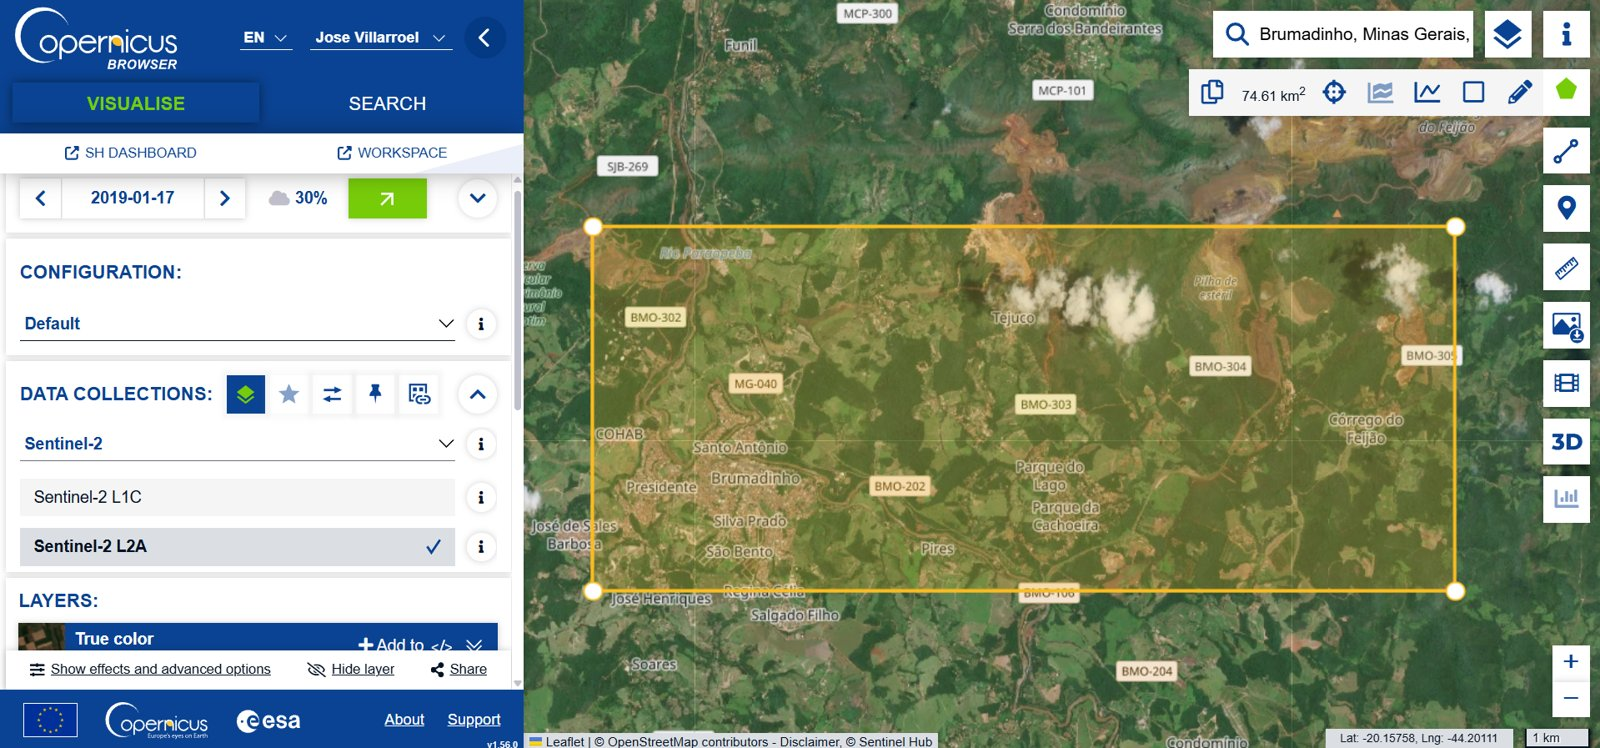
\includegraphics[width=0.85\textwidth]{figures/copernicus_aoi}
 \caption{Área de descarga (74{,}61\,km$^2$) definida en Copernicus Browser.}
 \label{fig:aoi}
\end{figure}

\section{Metodología}
La implementación sigue un flujo estructurado de cinco fases \parencite{Lillesand2015}. Esta entrega documenta las fases 1 a 3. Todo el procesamiento se realizó en QGIS \parencite{QGIS_Software}.

\subsection{Fase 1: Definición del problema y adquisición de datos}
\begin{itemize}
    \item \textbf{Fechas:} Se revisaron en Copernicus Browser las adquisiciones disponibles alrededor del evento, aplicando un filtro de nubosidad máxima del 30\,\%. El criterio de selección fue elegir las escenas más próximas al evento en las que el ROI estuviera libre de nubes. Esto minimiza los cambios ajenos al fenómeno, como la fenología o los cambios de uso del suelo.
    \begin{itemize}
        \item $t_1$ (antes): \textbf{17 de enero de 2019} (Figura~\ref{fig:copernicus}a).
        \item $t_2$ (después): \textbf{1 de febrero de 2019} (Figura~\ref{fig:copernicus}b).
    \end{itemize}
    El intervalo es de 15 días, suficientemente corto para atribuir los cambios principales al evento.
    \item \textbf{Fuente de datos:} Se usaron imágenes ópticas Sentinel-2 MSI de nivel 2A. Se descargaron por la pestaña \emph{Analytical} de Copernicus Browser (Figura~\ref{fig:descarga}) con los siguientes parámetros:
    \begin{itemize}
        \item formato TIFF de 16 bits y resolución HIGH (1416$\times$598 píxeles);
        \item sistema de referencia WGS84 (EPSG:4326);
        \item tamaño de píxel de $8{,}98\times10^{-5}\,^\circ$ en longitud y $8{,}43\times10^{-5}\,^\circ$ en latitud, equivalente a $\approx$9{,}4\,m$\times$9{,}3\,m a esta latitud.
    \end{itemize}
    Se descargaron tres bandas crudas, todas con resolución nativa de 10\,m: B03 (verde, 560\,nm), B04 (rojo, 665\,nm) y B08 (infrarrojo cercano, 842\,nm). También se descargaron la composición en color verdadero y la capa de clasificación de escena (SCL), usada para el control de calidad.
    \item \textbf{SAR:} No se empleó Sentinel-1, porque ambas fechas ópticas presentan el ROI despejado.
    \item \textbf{Definición del ROI:} El proyecto de QGIS se configuró en WGS84/UTM zona 23S (EPSG:32723) para trabajar en unidades métricas (Figura~\ref{fig:src}). Luego se creó el GeoPackage \texttt{ROI\_Brumadinho} (Figura~\ref{fig:gpkg}) y se digitalizó el polígono sobre la imagen $t_2$ (Figura~\ref{fig:roi}). Finalmente, se simplificó con el algoritmo de Douglas-Peucker con una tolerancia de 15\,m (Figura~\ref{fig:simplificar}). Así se reduce el número de vértices sin perder la forma del corredor.
\end{itemize}

\begin{figure}[H]
 \centering
 \begin{subfigure}{0.49\textwidth}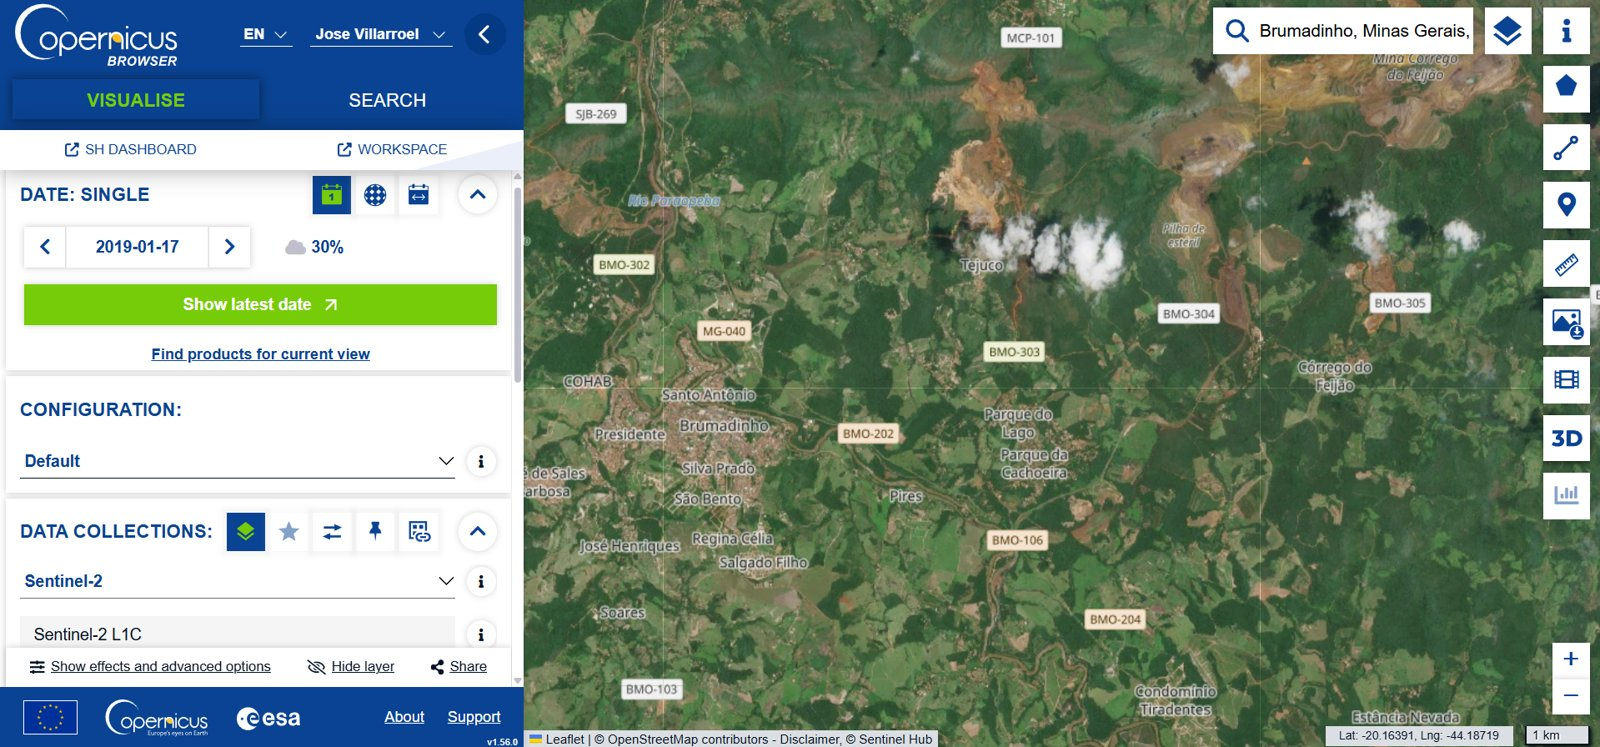
\includegraphics[width=\linewidth]{figures/copernicus_t1}\caption{$t_1$: 17-01-2019}\end{subfigure}
 \hfill
 \begin{subfigure}{0.49\textwidth}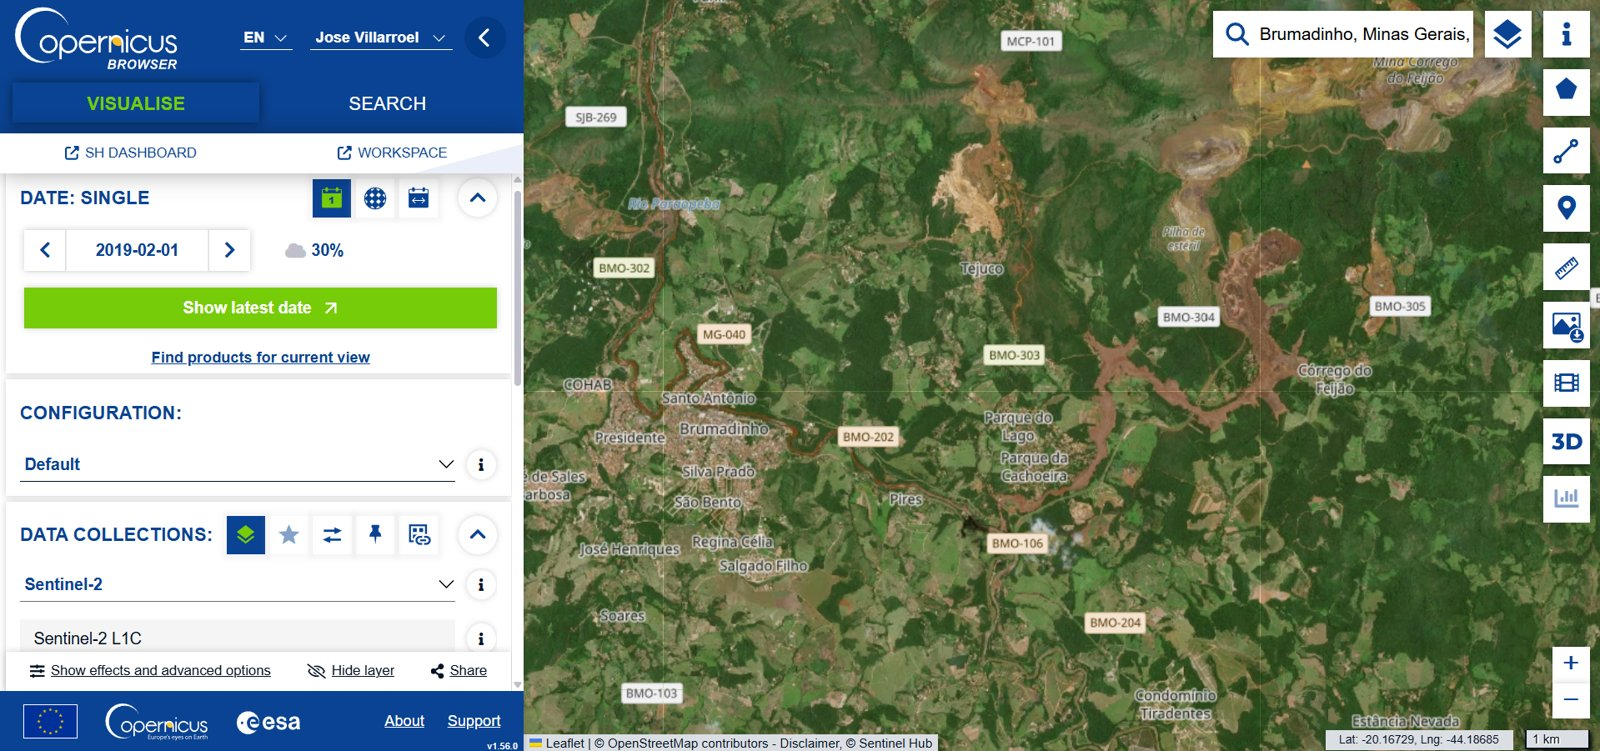
\includegraphics[width=\linewidth]{figures/copernicus_t2}\caption{$t_2$: 01-02-2019}\end{subfigure}
 \caption{Selección de las fechas $t_1$ y $t_2$ en Copernicus Browser.}
 \label{fig:copernicus}
\end{figure}

\begin{figure}[H]
 \centering
 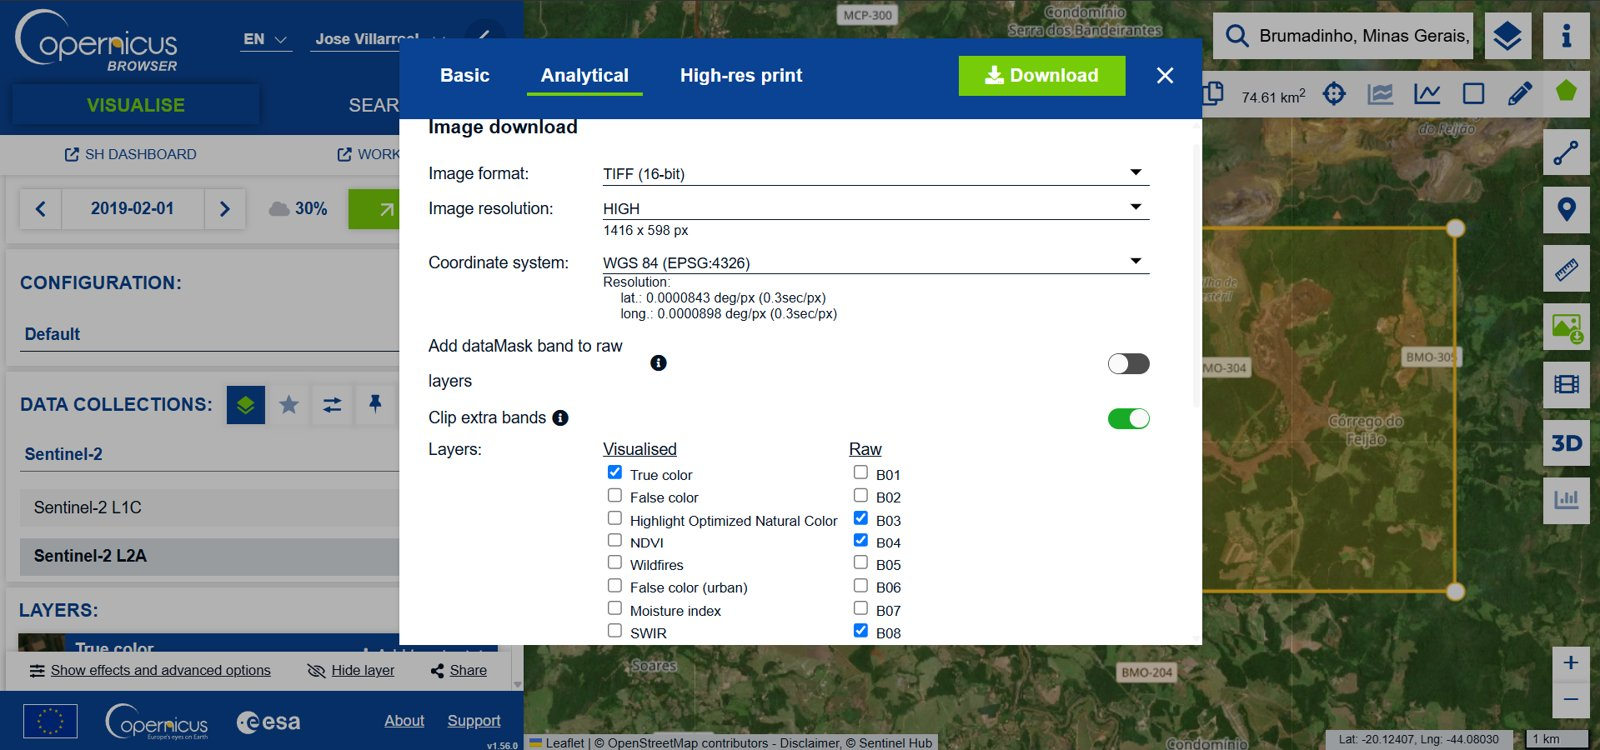
\includegraphics[width=0.8\textwidth]{figures/descarga_bandas}
 \caption{Parámetros de descarga analítica: TIFF 16 bits, EPSG:4326 y bandas B03, B04 y B08.}
 \label{fig:descarga}
\end{figure}

\begin{figure}[H]
 \centering
 \begin{subfigure}{0.49\textwidth}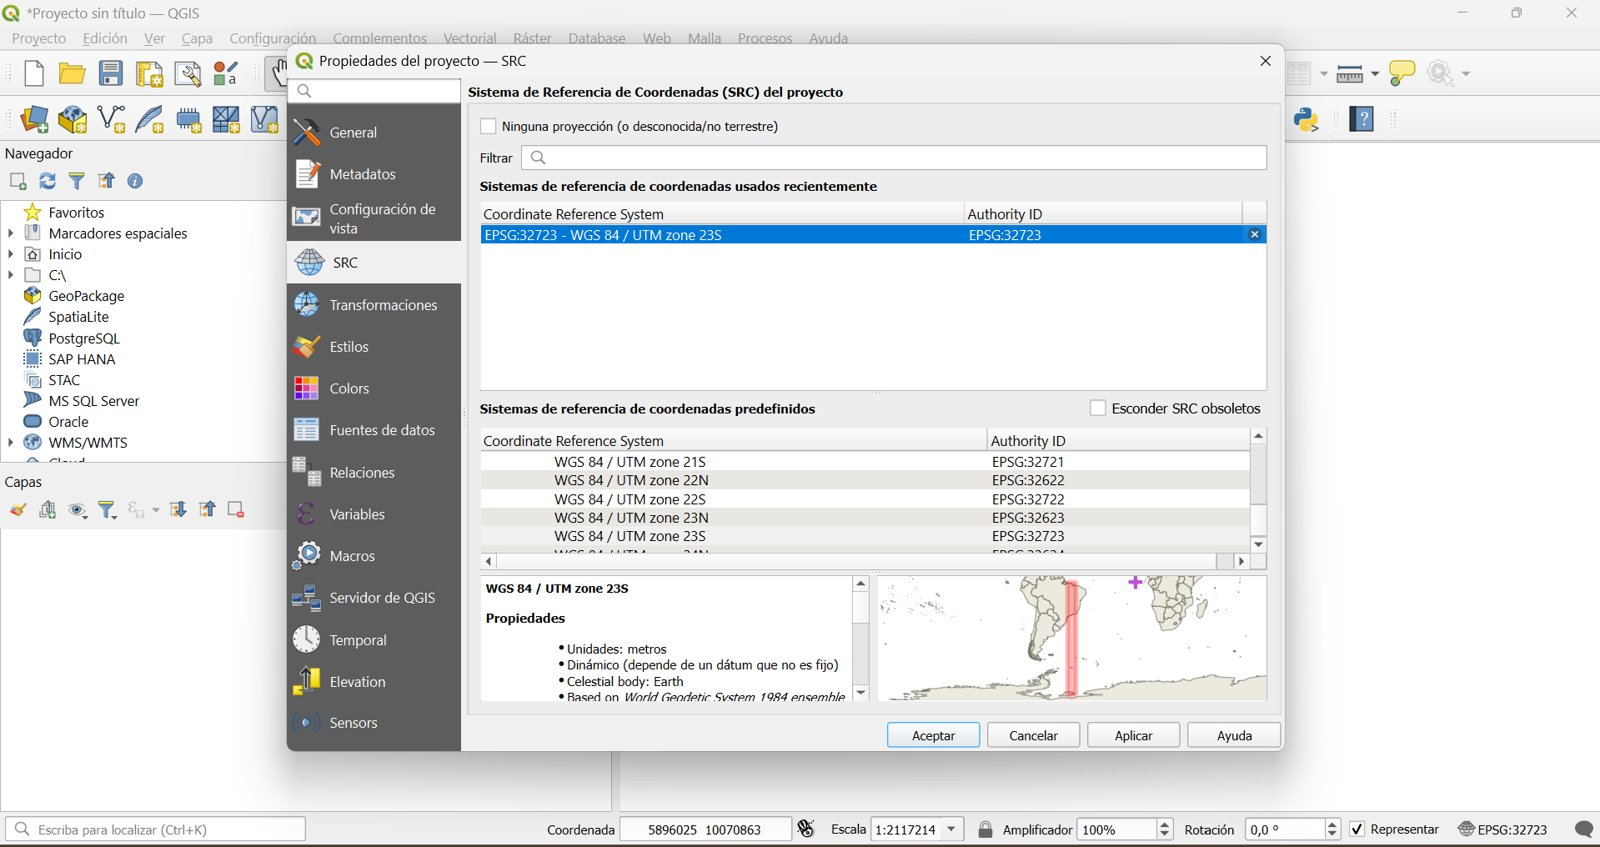
\includegraphics[width=\linewidth]{figures/src_proyecto}\caption{SRC del proyecto (EPSG:32723)}\label{fig:src}\end{subfigure}
 \hfill
 \begin{subfigure}{0.49\textwidth}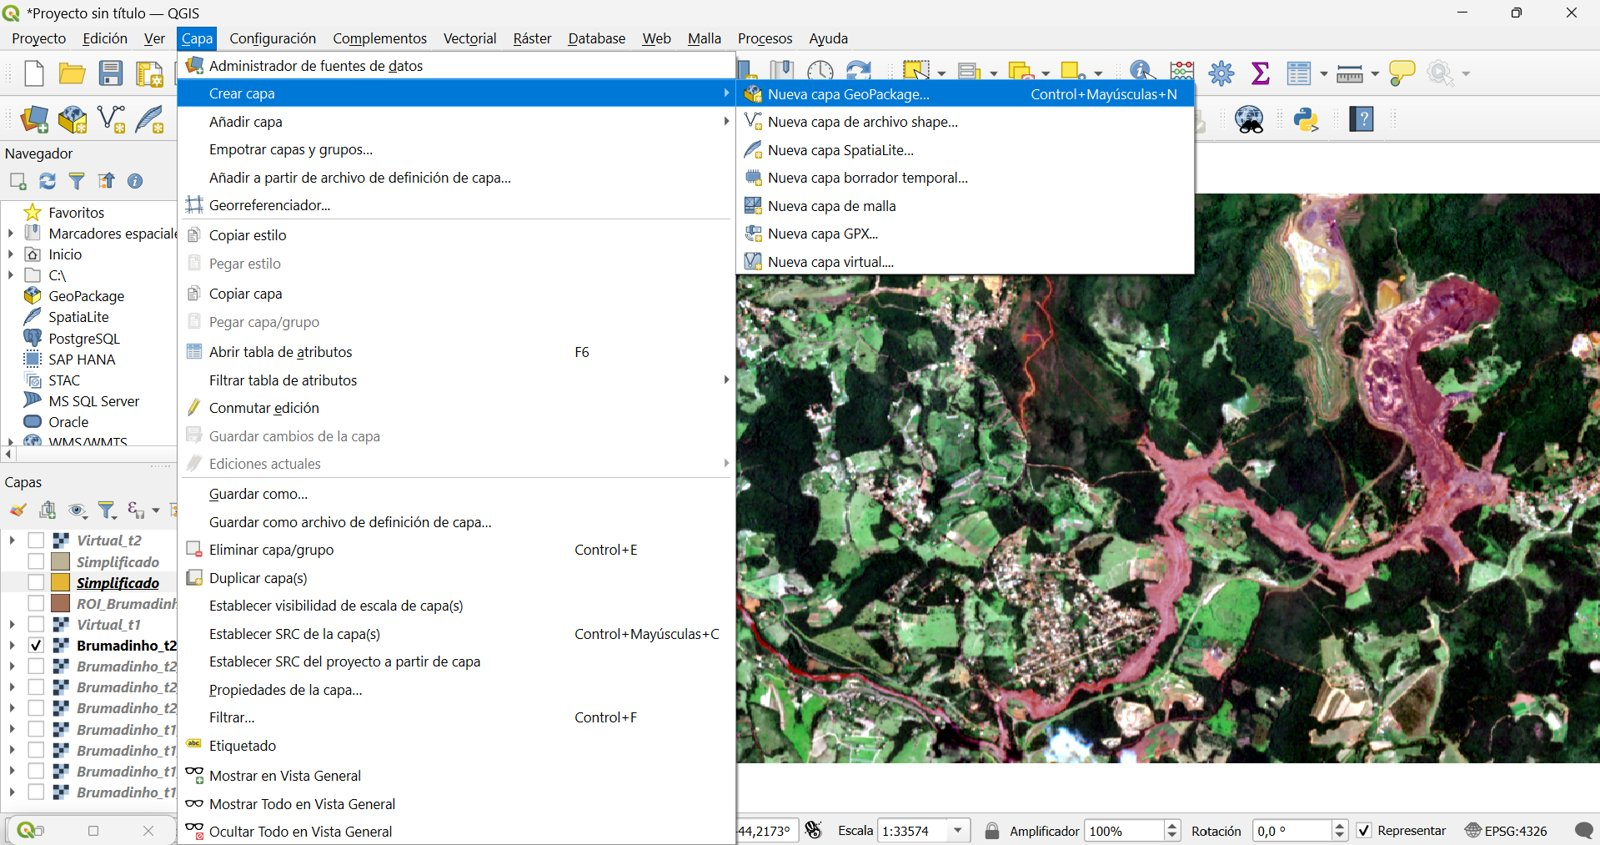
\includegraphics[width=\linewidth]{figures/crear_gpkg}\caption{Creación del GeoPackage}\label{fig:gpkg}\end{subfigure}
 \caption{Configuración del proyecto en QGIS.}
\end{figure}

\begin{figure}[H]
 \centering
 \begin{subfigure}{0.49\textwidth}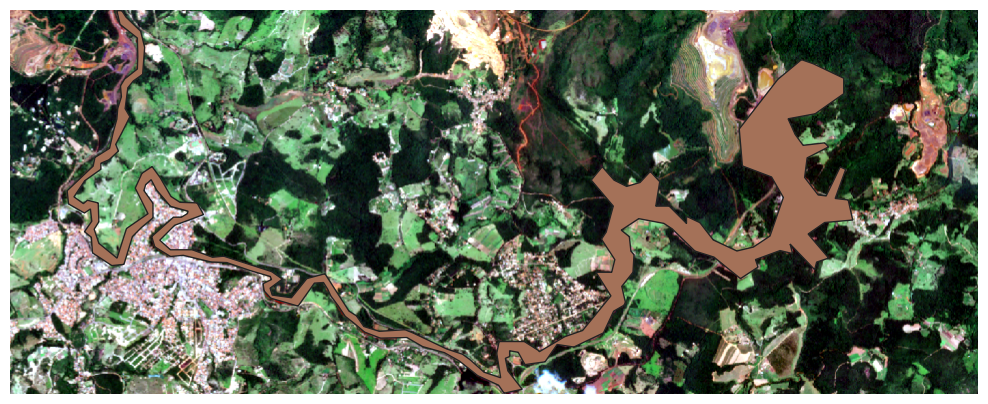
\includegraphics[width=\linewidth]{figures/roi}\caption{ROI digitalizado sobre $t_2$}\label{fig:roi}\end{subfigure}
 \hfill
 \begin{subfigure}{0.49\textwidth}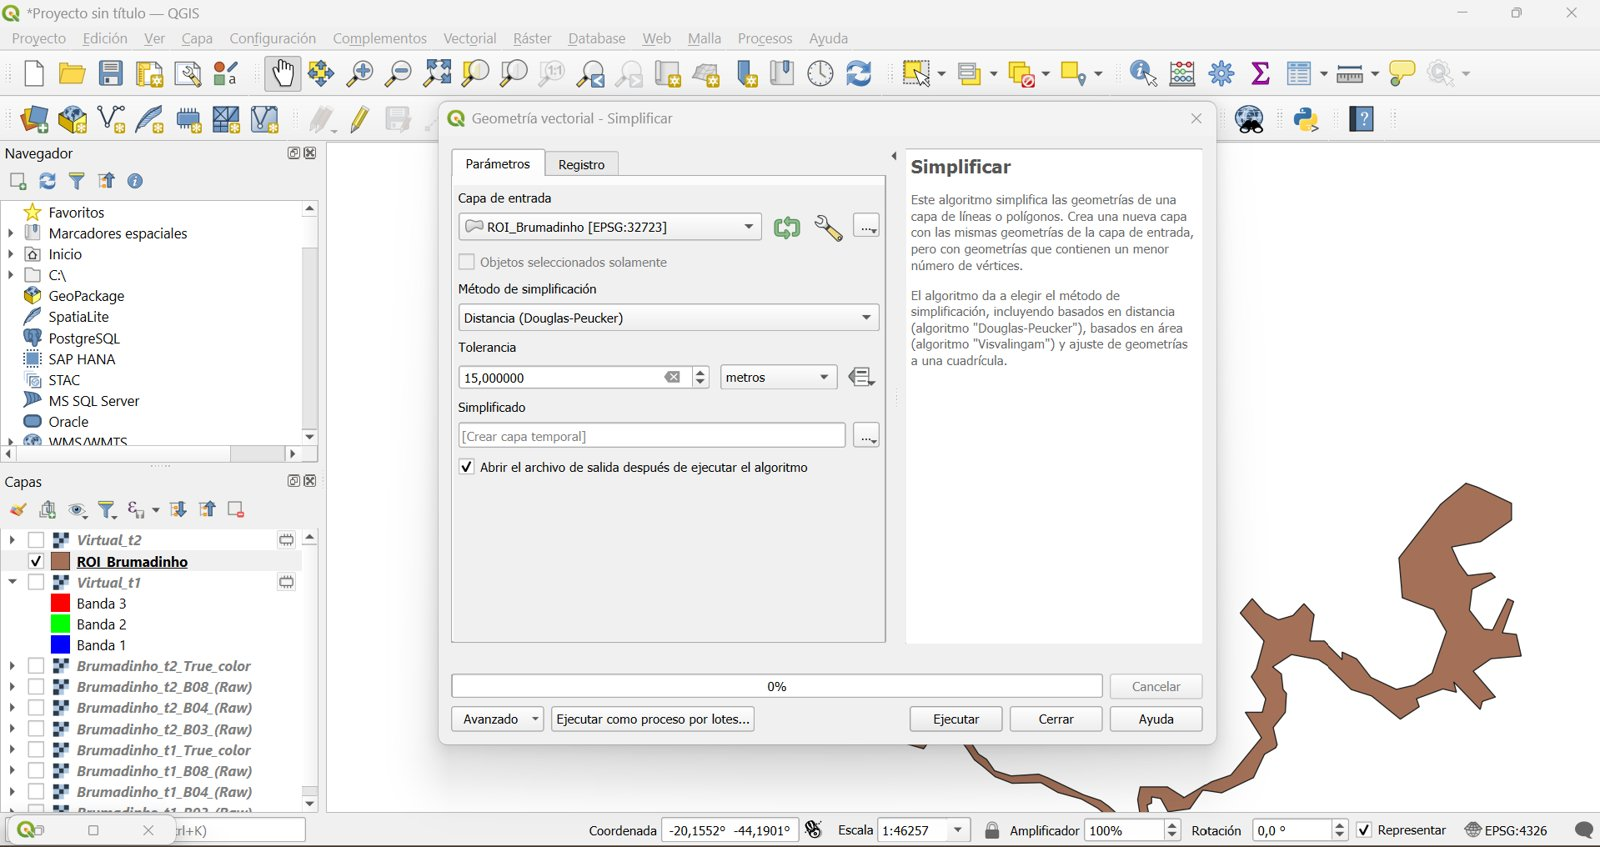
\includegraphics[width=\linewidth]{figures/simplificar}\caption{Simplificación Douglas-Peucker}\label{fig:simplificar}\end{subfigure}
 \caption{Definición del ROI.}
\end{figure}

\subsection{Fase 2: Preprocesamiento}
Antes de comparar dos imágenes es necesario que sean radiométrica y geométricamente comparables. De lo contrario, las diferencias entre ellas podrían deberse a la atmósfera, a desplazamientos de la malla o a nubes, y no a cambios reales en la superficie \parencite{Singh1989}. Se aplicaron los siguientes pasos.
\begin{itemize}
    \item \textbf{Corrección atmosférica:} Ambas escenas corresponden al producto Sentinel-2 L2A, es decir, reflectancia en la superficie o \emph{Bottom-of-Atmosphere} (BOA). Este producto se genera con el procesador Sen2Cor, que corrige la dispersión y la absorción atmosféricas \parencite{MainKnorn2017}, por lo que no se requirió una corrección adicional. Los valores se almacenan como enteros de 16 bits escalados (reflectancia $\times$ 10\,000). Como NDVI y NDWI son cocientes normalizados, el factor de escala se cancela y no afecta los resultados.
    \item \textbf{Co-registro:} Se verificó en las propiedades de cada capa (Propiedades $\rightarrow$ Información, Figura~\ref{fig:coreg}). Las capas de $t_1$ y $t_2$ comparten:
    \begin{itemize}
        \item el mismo SRC (EPSG:4326);
        \item la misma extensión;
        \item el mismo número de filas y columnas (1416$\times$598);
        \item el mismo tipo de dato (UInt16).
    \end{itemize}
    Como ambas imágenes provienen del mismo sensor y de la misma malla de remuestreo, cada píxel de $t_1$ corresponde exactamente al mismo lugar en $t_2$. Como verificación visual se construyeron rásteres virtuales con las bandas B03, B04 y B08 (Ráster $\rightarrow$ Miscelánea $\rightarrow$ Construir ráster virtual; Figuras~\ref{fig:vrt} y \ref{fig:simbologia}). Estos se visualizaron en falso color infrarrojo (R=B08, G=B04, B=B03). En la Figura~\ref{fig:falsecolor} se aprecia que carreteras, cauces y límites de parcelas coinciden en ambas fechas.
    \item \textbf{Remuestreo:} No fue necesario. Ambas fechas provienen del mismo sensor (MSI) y todas las bandas usadas tienen la misma resolución nativa (10\,m) y la misma malla de salida.
    \item \textbf{Recorte al ROI:} Cada banda se recortó con el polígono del ROI mediante Ráster $\rightarrow$ Extracción $\rightarrow$ Cortar ráster por capa de máscara (Figura~\ref{fig:clip}). El resultado fueron las capas \texttt{t1\_B03\_clip}, \texttt{t1\_B04\_clip}, \texttt{t1\_B08\_clip} y \texttt{t1\_SCL\_clip}, y sus equivalentes para $t_2$. El recorte reduce el tiempo de procesamiento y concentra el análisis en la zona de interés.
    \item \textbf{Enmascaramiento de nubes:} Se utilizó la banda de control de calidad SCL (\emph{Scene Classification Layer}) de Sen2Cor. Con la calculadora ráster se generó una máscara binaria que marca como inválidos los píxeles de las clases 0 (sin datos), 1 (saturado o defectuoso), 3 (sombra de nube), 8 (nube de probabilidad media), 9 (nube de probabilidad alta) y 10 (cirros):
    \begin{equation}
     M = (\mathrm{SCL}=0) \lor (\mathrm{SCL}=1) \lor (\mathrm{SCL}=3) \lor (\mathrm{SCL}=8) \lor (\mathrm{SCL}=9) \lor (\mathrm{SCL}=10)
    \end{equation}
    Las máscaras \texttt{t1\_cloudmask} y \texttt{t2\_cloudmask} (Figura~\ref{fig:cloudmask}) toman el valor 0 en todo el ROI. Esto indica que no hay píxeles afectados por nubes ni sombras dentro del área de análisis. Las nubes presentes en $t_1$ se localizan al norte, fuera del polígono (Figura~\ref{fig:falsecolor}a).
\end{itemize}

\begin{figure}[H]
 \centering
 \begin{subfigure}{0.49\textwidth}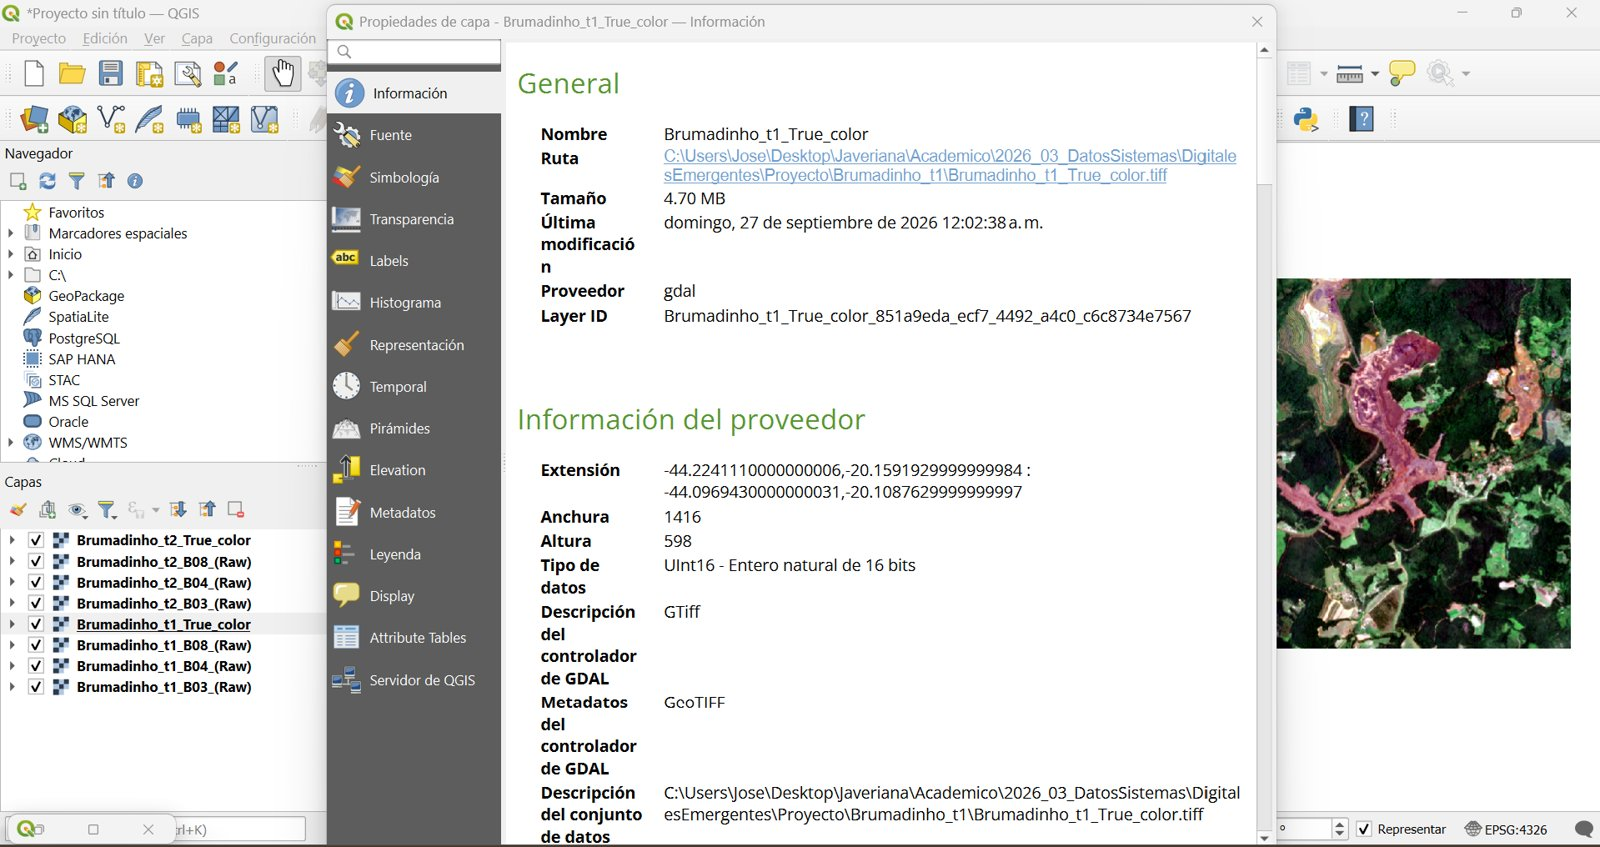
\includegraphics[width=\linewidth]{figures/coreg_t1}\caption{$t_1$}\end{subfigure}
 \hfill
 \begin{subfigure}{0.49\textwidth}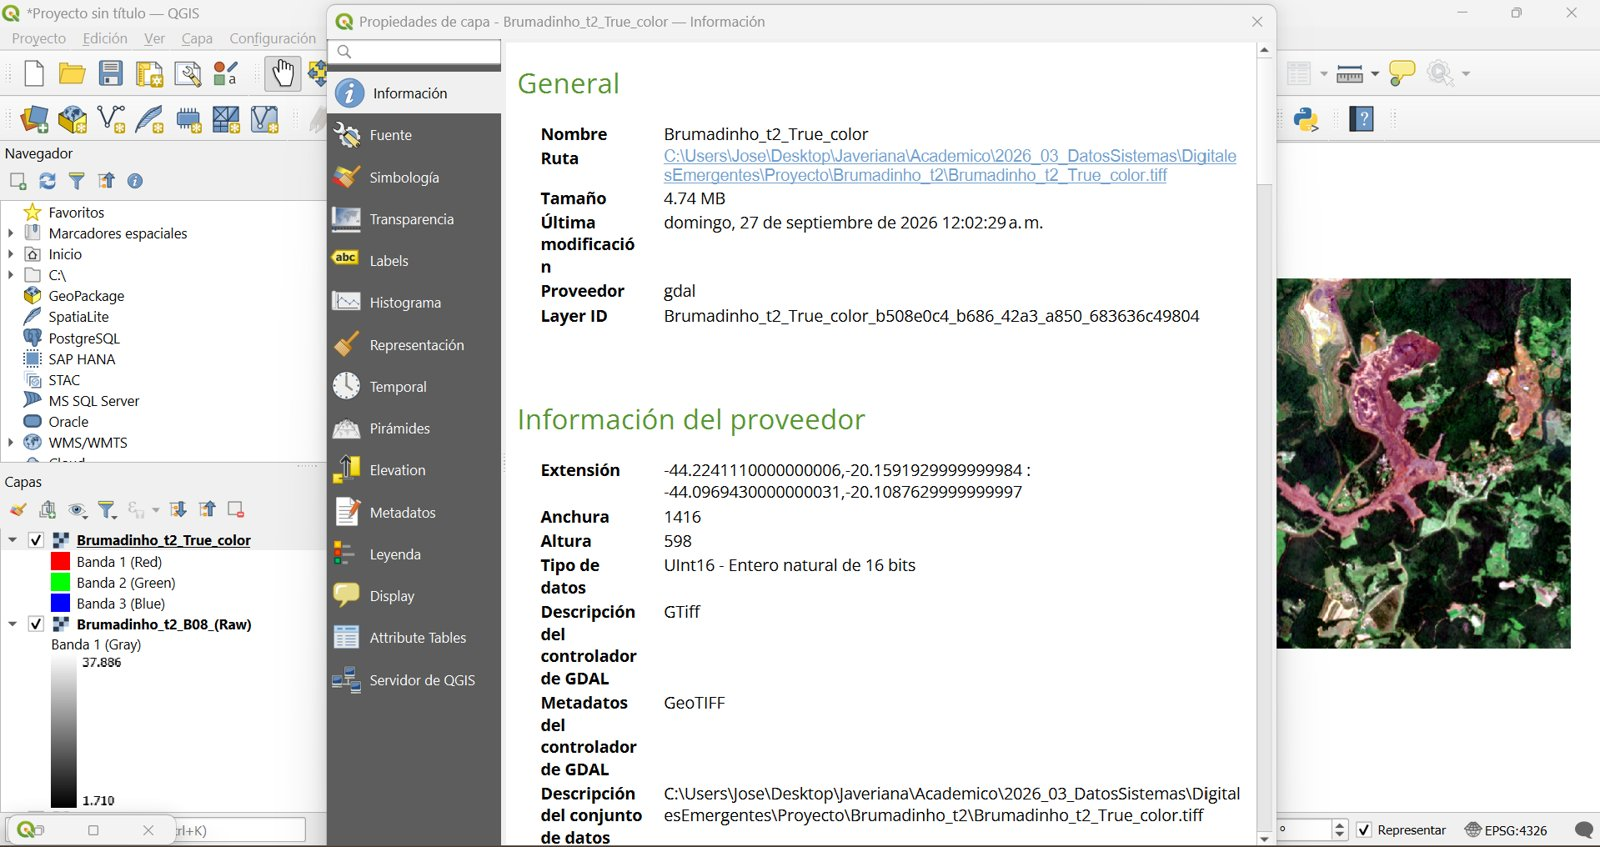
\includegraphics[width=\linewidth]{figures/coreg_t2}\caption{$t_2$}\end{subfigure}
 \caption{Verificación de co-registro: extensión, dimensiones y tipo de dato idénticos en ambas fechas.}
 \label{fig:coreg}
\end{figure}

\begin{figure}[H]
 \centering
 \begin{subfigure}{0.49\textwidth}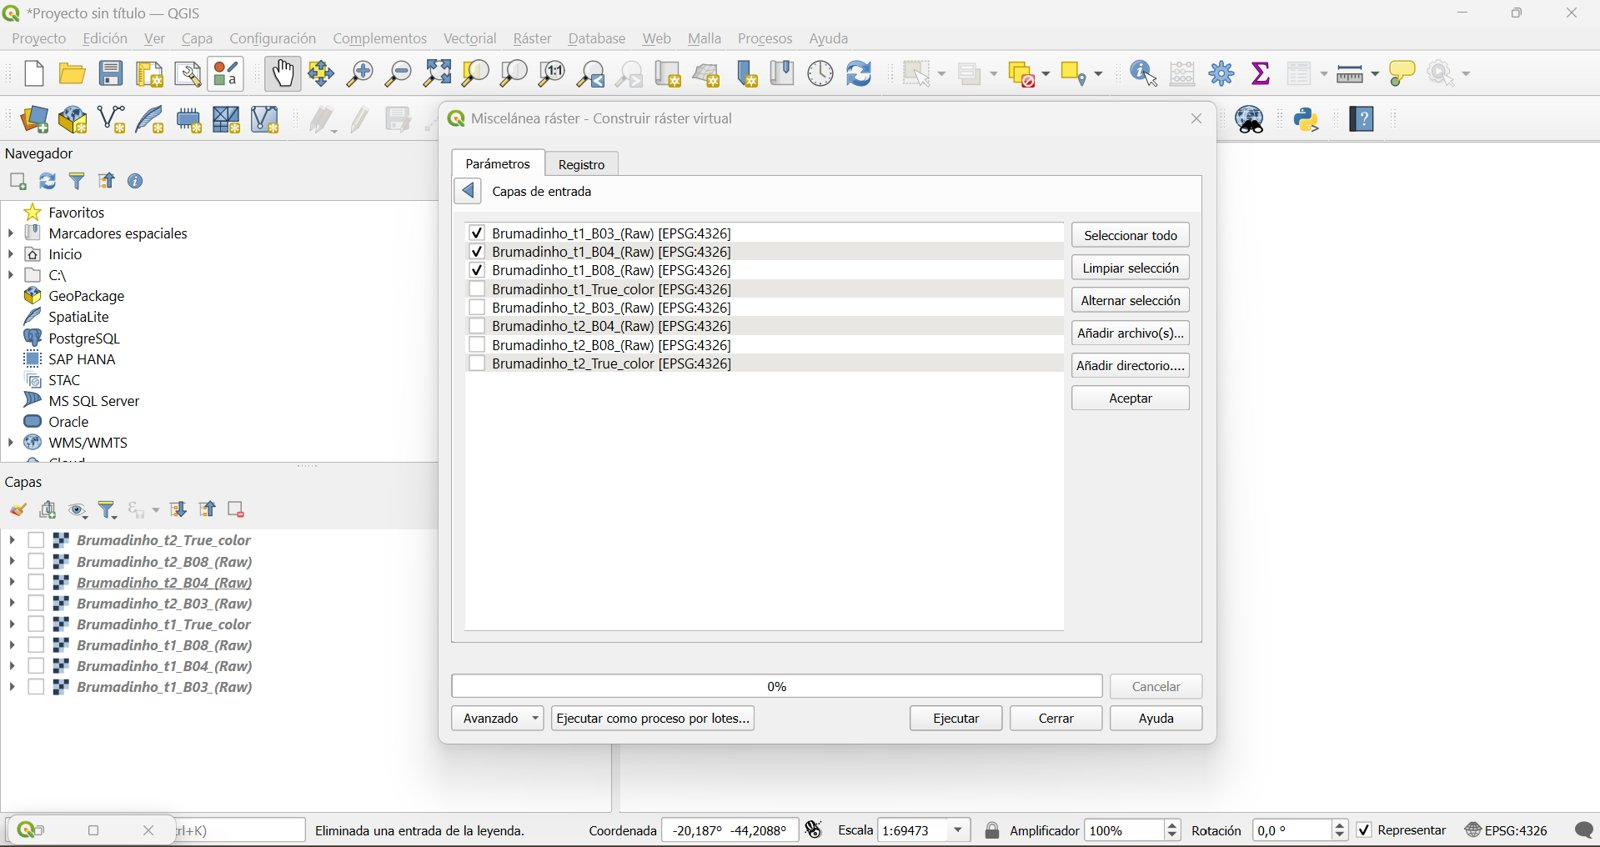
\includegraphics[width=\linewidth]{figures/vrt_bandas}\caption{Selección de bandas}\label{fig:vrt}\end{subfigure}
 \hfill
 \begin{subfigure}{0.49\textwidth}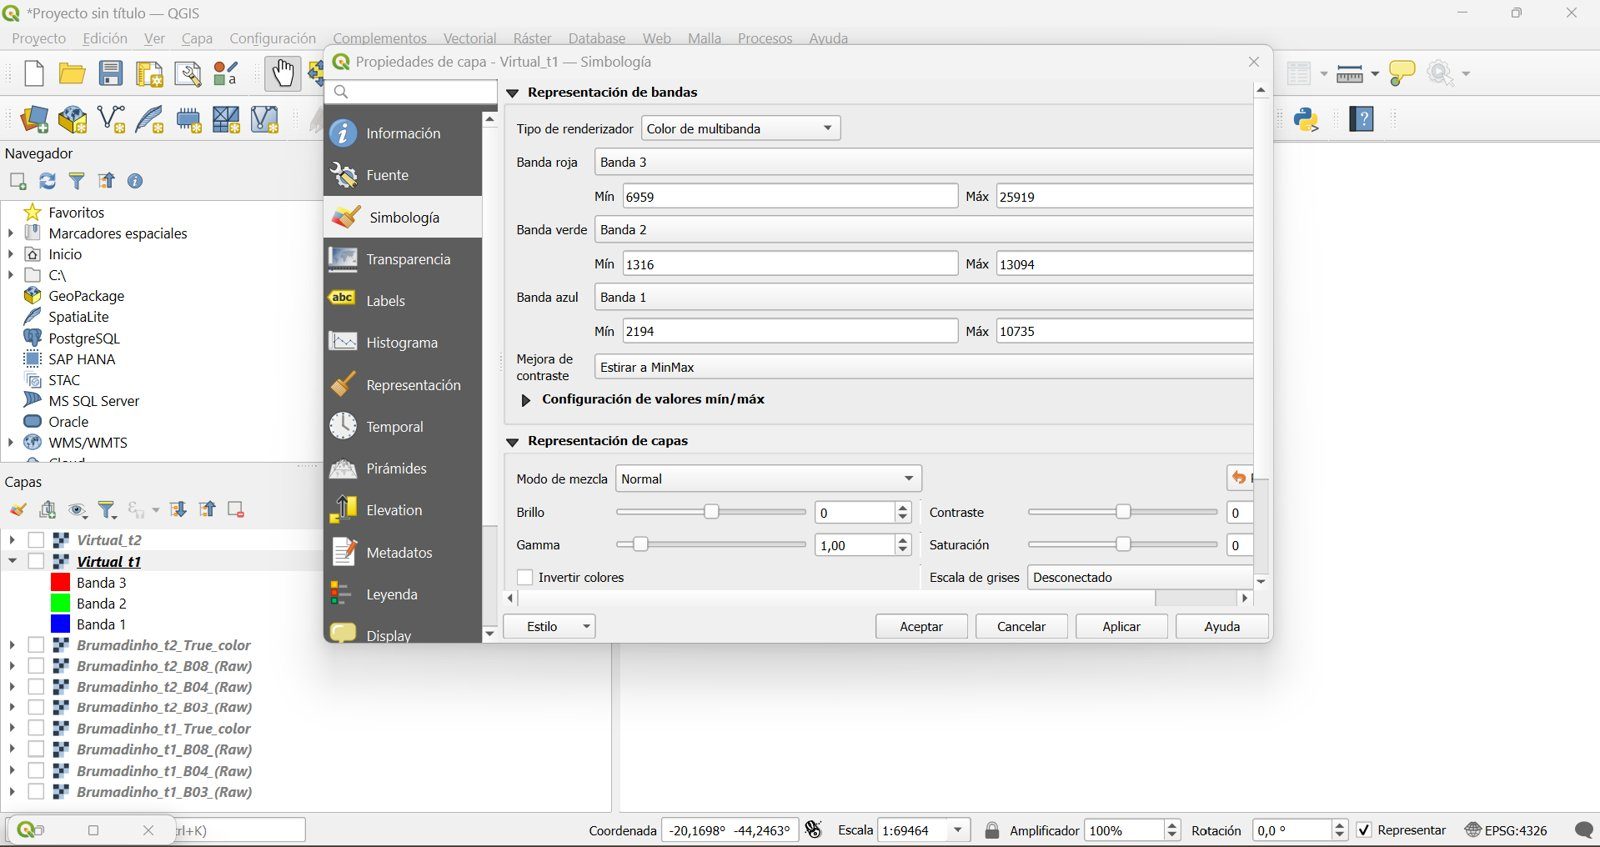
\includegraphics[width=\linewidth]{figures/simbologia_vrt}\caption{Asignación de bandas RGB}\label{fig:simbologia}\end{subfigure}
 \caption{Construcción del ráster virtual y simbología en falso color.}
\end{figure}

\begin{figure}[H]
 \centering
 \begin{subfigure}{0.49\textwidth}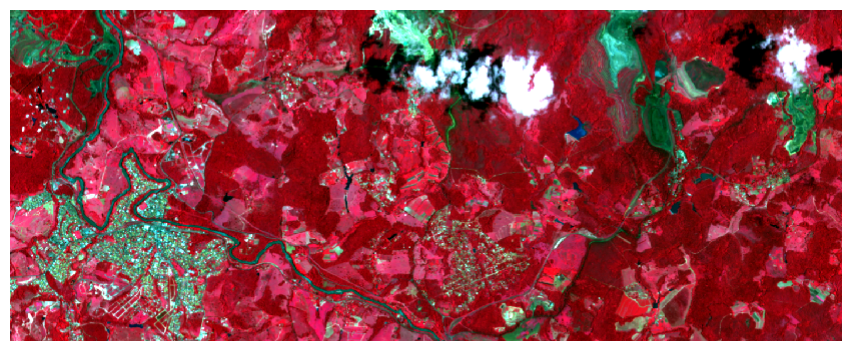
\includegraphics[width=\linewidth]{figures/falsecolor_t1}\caption{$t_1$ (17-01-2019)}\end{subfigure}
 \hfill
 \begin{subfigure}{0.49\textwidth}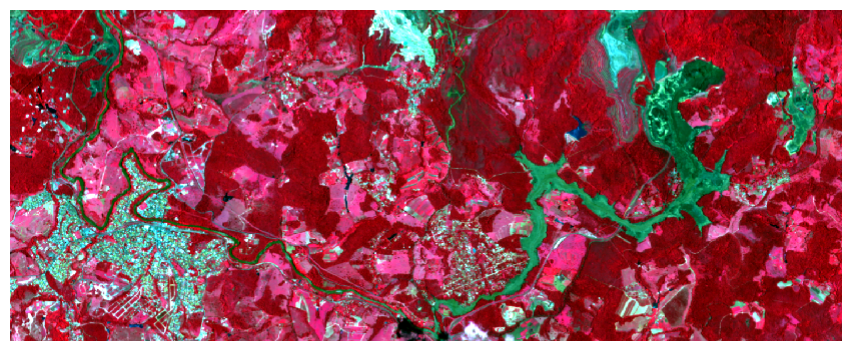
\includegraphics[width=\linewidth]{figures/falsecolor_t2}\caption{$t_2$ (01-02-2019)}\end{subfigure}
 \caption{Composición en falso color infrarrojo (R=B08, G=B04, B=B03). La vegetación aparece en rojo por su alta reflectancia en el NIR. En $t_2$ el material depositado aparece en tonos verde-cian a lo largo del valle, donde en $t_1$ había vegetación.}
 \label{fig:falsecolor}
\end{figure}

\begin{figure}[H]
 \centering
 \begin{subfigure}{0.49\textwidth}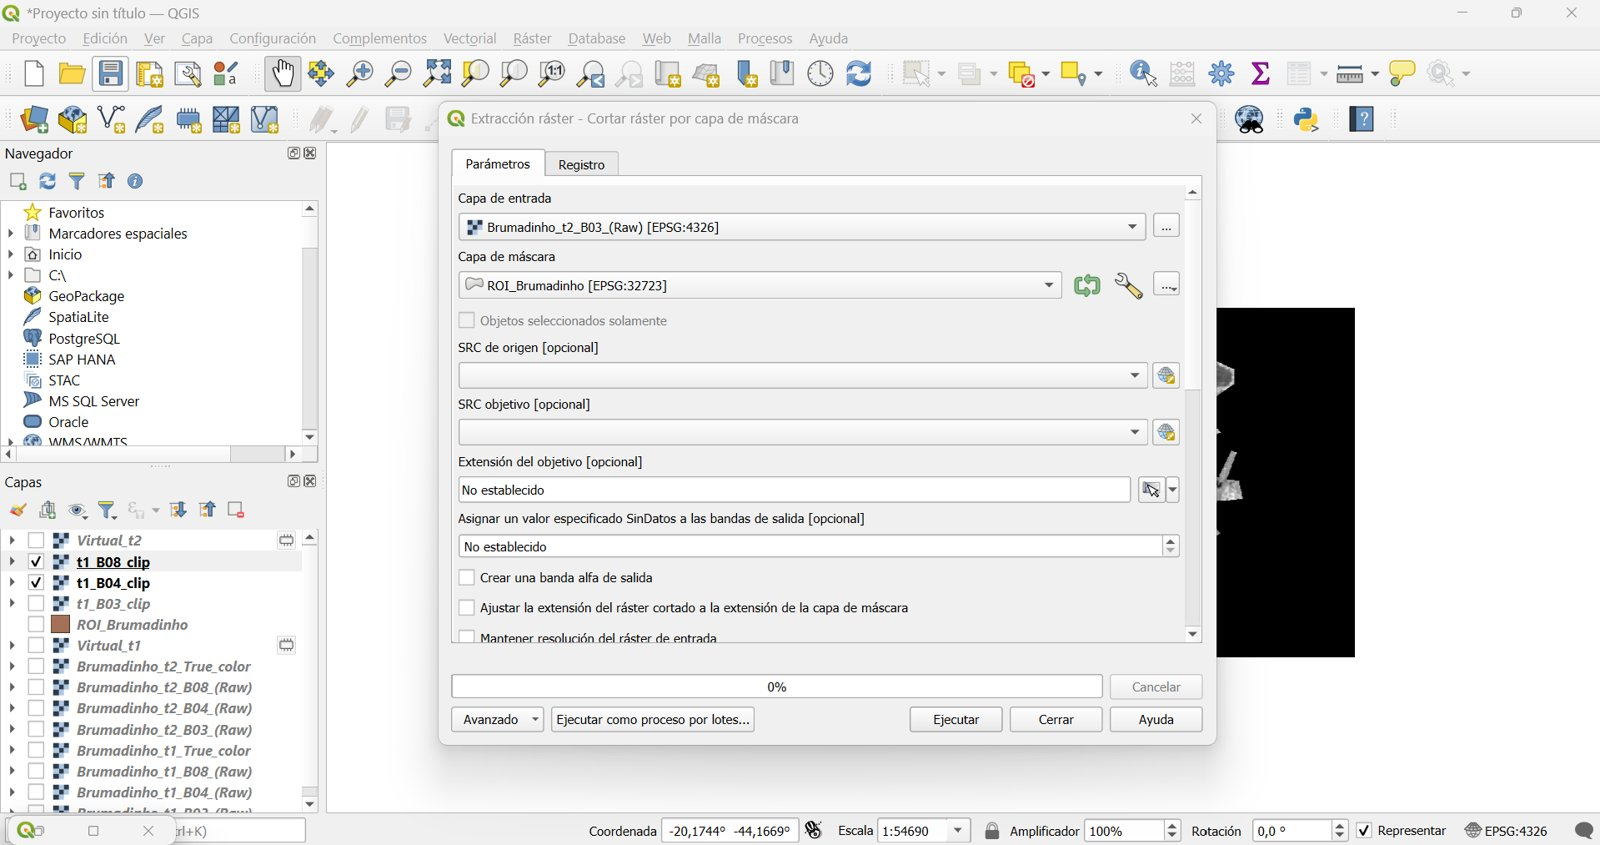
\includegraphics[width=\linewidth]{figures/clip_param}\caption{Parámetros del recorte}\end{subfigure}
 \hfill
 \begin{subfigure}{0.49\textwidth}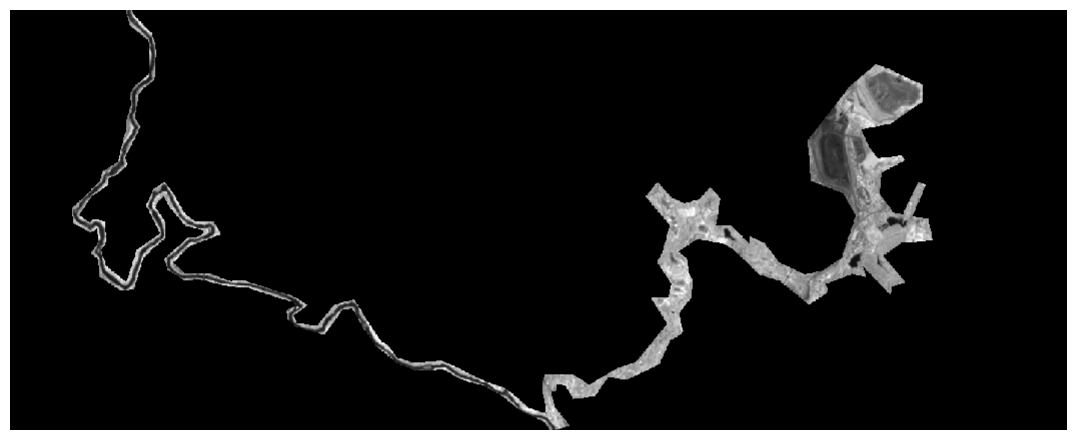
\includegraphics[width=\linewidth]{figures/clip_result}\caption{Banda recortada}\end{subfigure}
 \caption{Recorte de las bandas con el polígono del ROI.}
 \label{fig:clip}
\end{figure}

\begin{figure}[H]
 \centering
 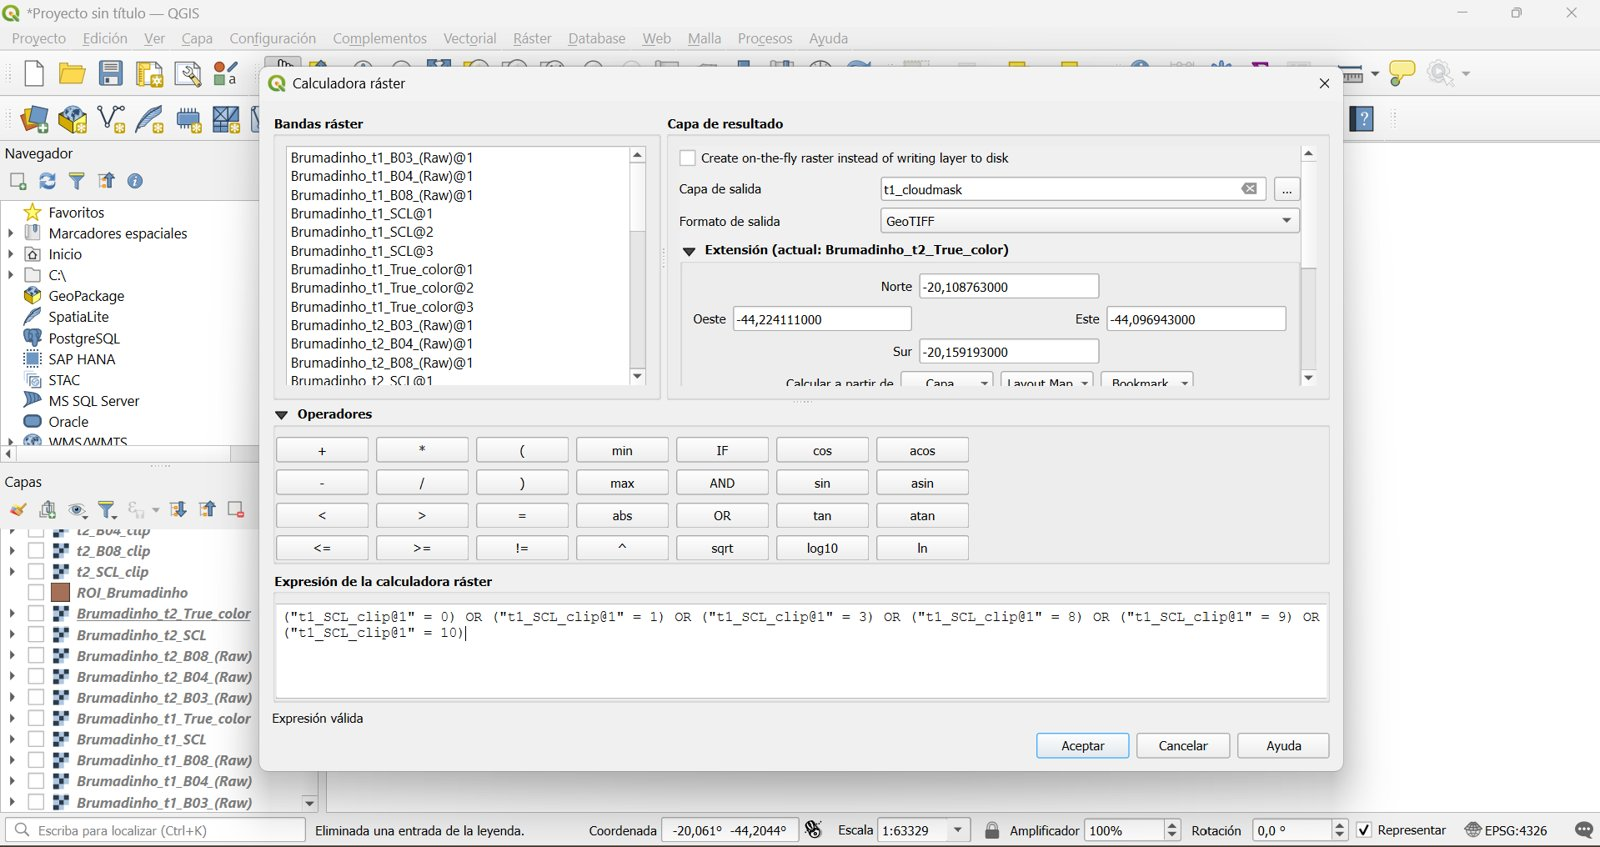
\includegraphics[width=0.75\textwidth]{figures/cloudmask_expr}\\[4pt]
 \begin{subfigure}{0.45\textwidth}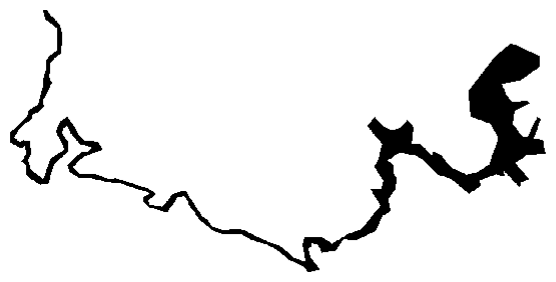
\includegraphics[width=\linewidth]{figures/cloudmask_t1}\caption{Máscara $t_1$}\end{subfigure}
 \hfill
 \begin{subfigure}{0.45\textwidth}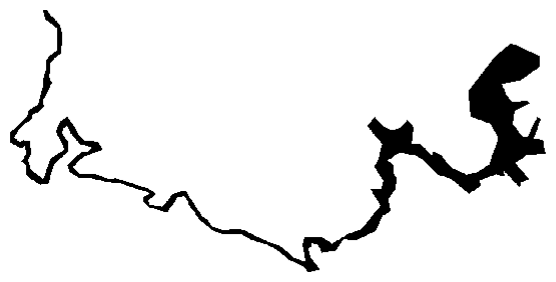
\includegraphics[width=\linewidth]{figures/cloudmask_t2}\caption{Máscara $t_2$}\end{subfigure}
 \caption{Máscara de nubes a partir de la banda SCL. El valor 0 (negro) en todo el ROI indica ausencia de nubes y sombras.}
 \label{fig:cloudmask}
\end{figure}

\subsection{Fase 3: Procesamiento y análisis de imágenes}
El cambio en el área de estudio tiene dos componentes principales:
\begin{itemize}
    \item la sustitución de coberturas vegetales por material mineral depositado;
    \item la alteración de la respuesta espectral del cauce por la carga de sedimentos.
\end{itemize}
Por ello se seleccionó el método de índices espectrales con diferenciación (Tabla~\ref{tab:techniques}), usando dos índices complementarios: uno orientado a la vegetación (NDVI) y otro al agua (NDWI).

\textbf{NDVI.} Se basa en el contraste entre la fuerte absorción de la clorofila en el rojo y la alta reflectancia del mesófilo foliar en el infrarrojo cercano \parencite{Rouse1974, Tucker1979}:
\begin{equation}
\mathrm{NDVI} = \frac{\rho_{NIR} - \rho_{Red}}{\rho_{NIR} + \rho_{Red}} = \frac{B08 - B04}{B08 + B04}
\end{equation}
Los valores altos (0{,}5--0{,}9) corresponden a vegetación densa y vigorosa. Los valores cercanos a 0 indican suelo desnudo o material mineral, y los valores negativos indican agua.

\textbf{NDWI.} Propuesto por \textcite{McFeeters1996}, maximiza la reflectancia del agua en el verde y minimiza su reflectancia en el infrarrojo cercano, donde el agua absorbe casi toda la radiación:
\begin{equation}
\mathrm{NDWI} = \frac{\rho_{Green} - \rho_{NIR}}{\rho_{Green} + \rho_{NIR}} = \frac{B03 - B08}{B03 + B08}
\end{equation}
Los valores positivos indican agua abierta, y los valores negativos indican vegetación o suelo.

\textbf{Diferencia de índices.} Para cada índice se calculó la diferencia entre fechas:
\begin{equation}
\Delta \text{Índice} = \text{Índice}_{t_2} - \text{Índice}_{t_1}
\end{equation}
Los valores negativos de $\Delta$NDVI indican pérdida de vegetación, y los valores negativos de $\Delta$NDWI indican disminución de la señal de agua. Los valores próximos a cero indican ausencia de cambio. Todos los cálculos se realizaron con la calculadora ráster de QGIS sobre las bandas recortadas (Figura~\ref{fig:expr}).

\begin{table}[H]
    \centering
    \caption{Metodologías de detección de cambios aplicadas}
    \label{tab:techniques}
    \begin{tabularx}{\textwidth}{lX}
        \toprule
        \textbf{Método} & \textbf{Técnica} \\
        \midrule
        Índices espectrales & Cálculo de NDVI (B08, B04) y NDWI (B03, B08) para $t_1$ y $t_2$. \\
        Diferencia de índices & $\Delta$NDVI y $\Delta$NDWI ($t_2 - t_1$) para localizar cambios de alta magnitud. \\
        Composición en falso color & Interpretación visual (R=B08, G=B04, B=B03) como apoyo cualitativo. \\
        \bottomrule
    \end{tabularx}
\end{table}

\begin{figure}[H]
 \centering
 \begin{subfigure}{0.49\textwidth}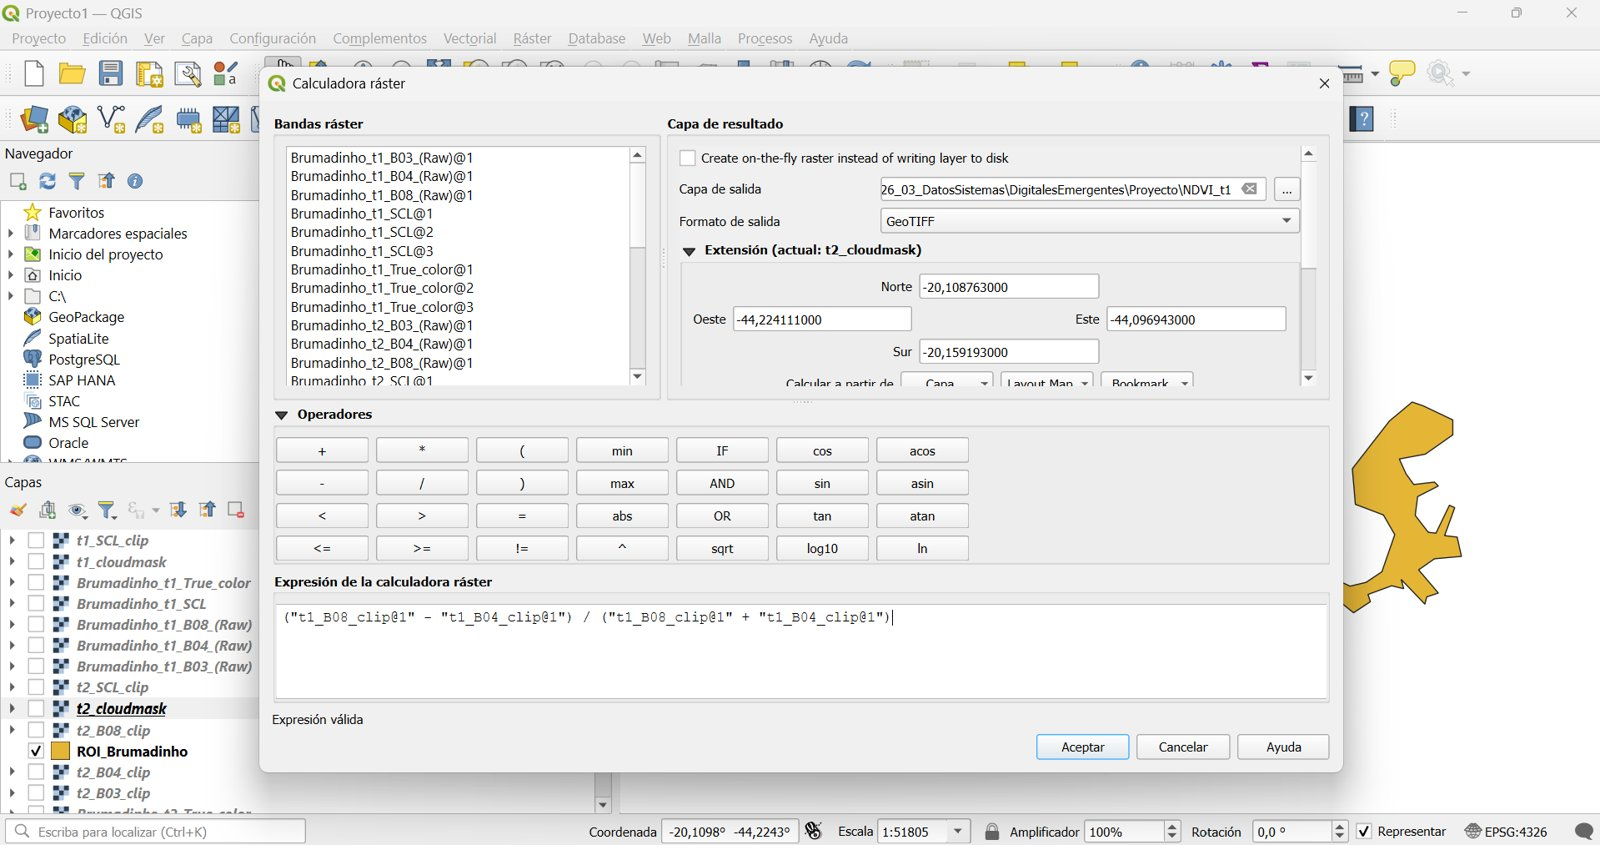
\includegraphics[width=\linewidth]{figures/ndvi_expr}\caption{NDVI}\end{subfigure}
 \hfill
 \begin{subfigure}{0.49\textwidth}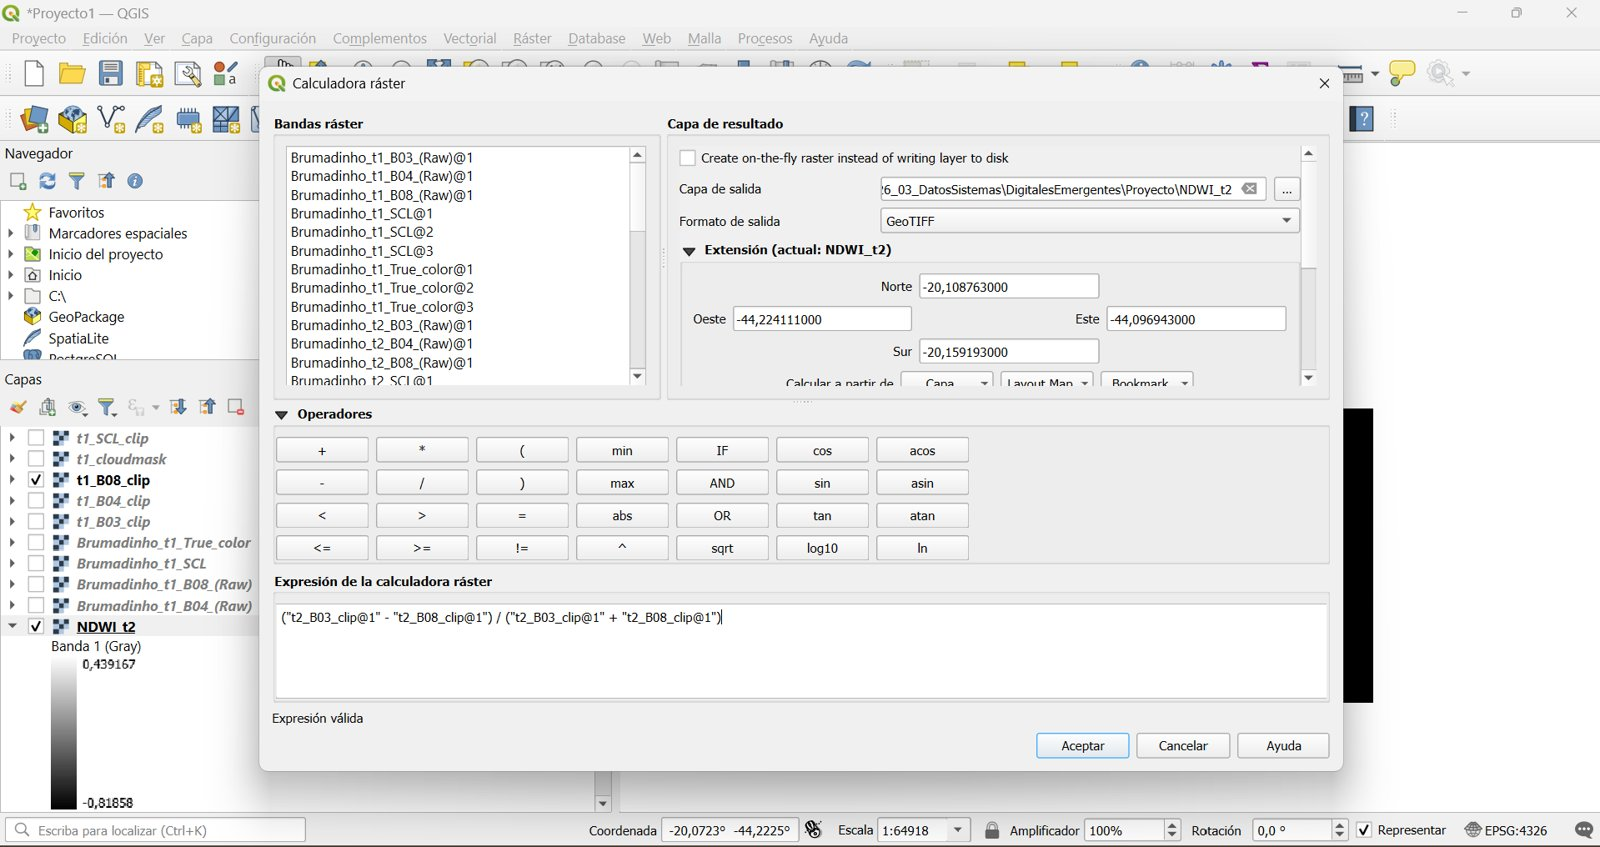
\includegraphics[width=\linewidth]{figures/ndwi_expr}\caption{NDWI}\end{subfigure}\\[4pt]
 \begin{subfigure}{0.49\textwidth}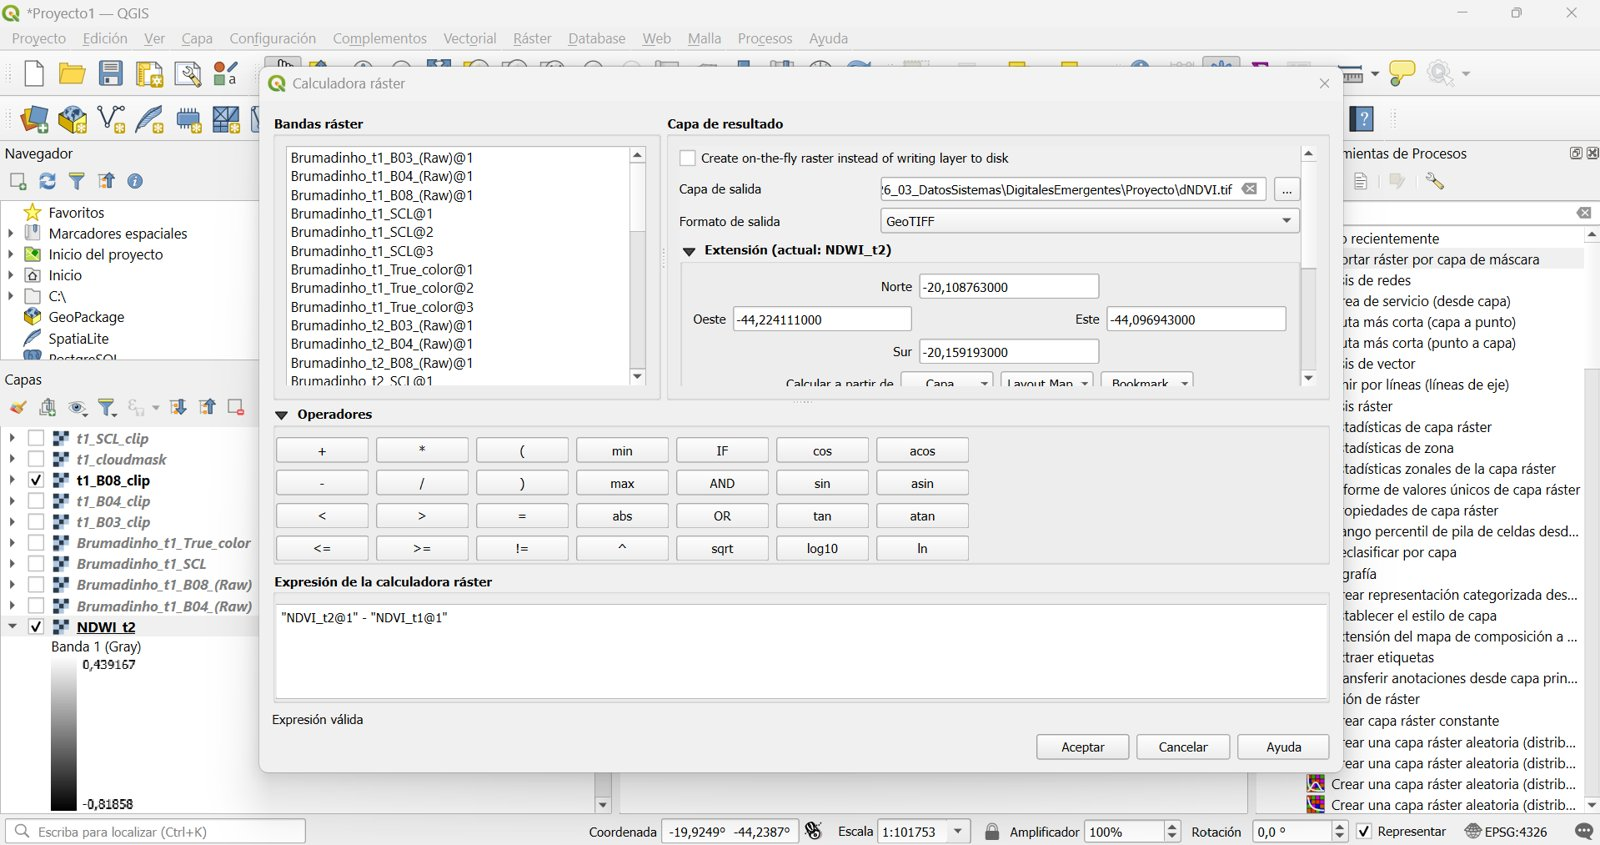
\includegraphics[width=\linewidth]{figures/dndvi_expr}\caption{$\Delta$NDVI}\end{subfigure}
 \hfill
 \begin{subfigure}{0.49\textwidth}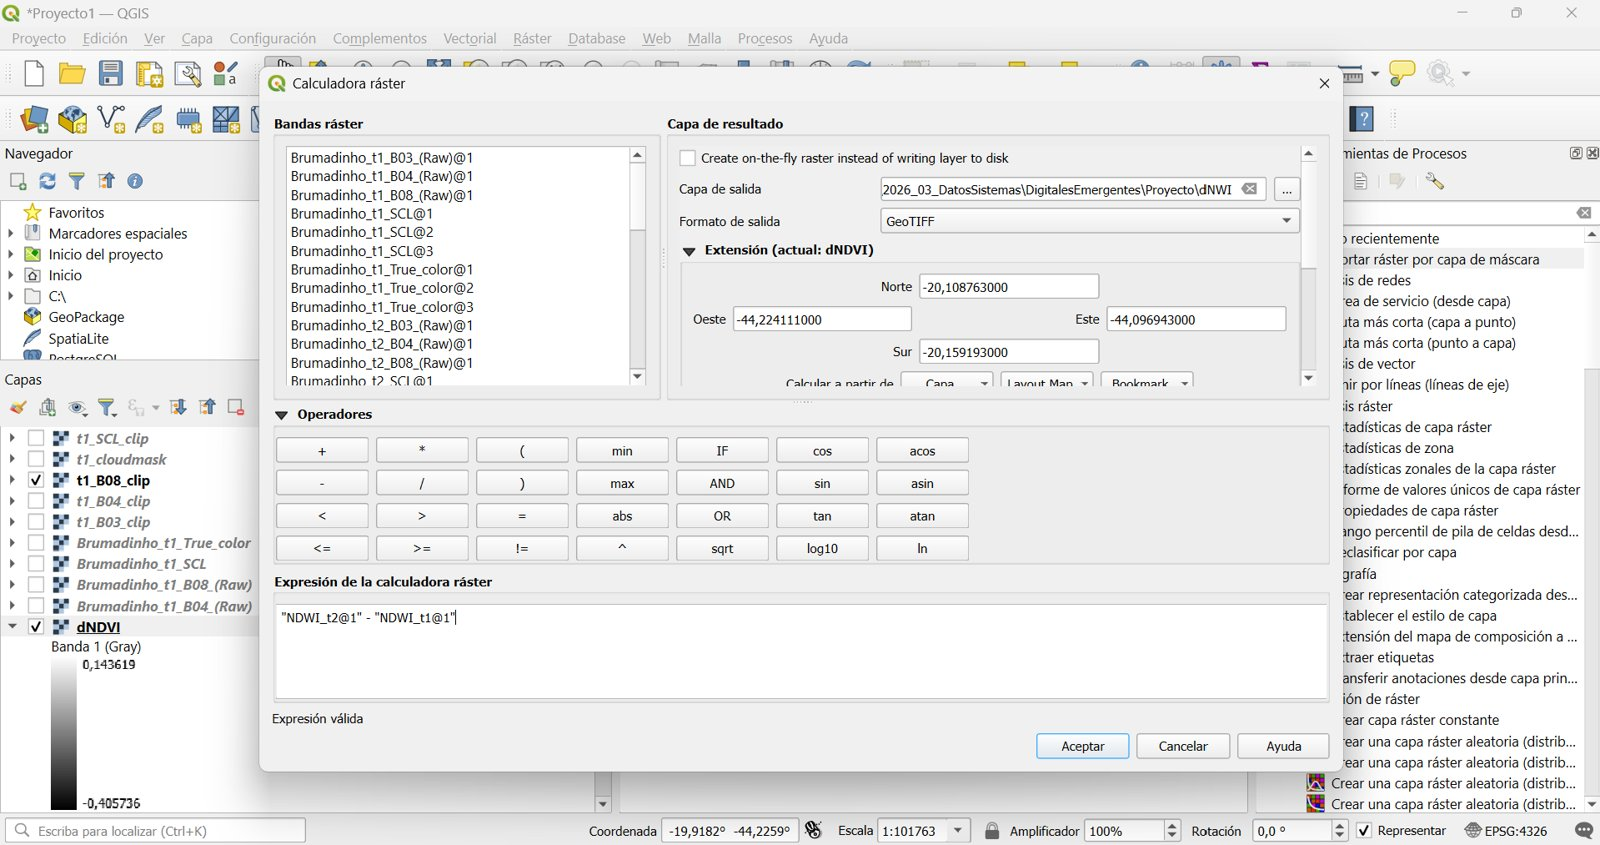
\includegraphics[width=\linewidth]{figures/dndwi_expr}\caption{$\Delta$NDWI}\end{subfigure}
 \caption{Expresiones empleadas en la calculadora ráster de QGIS.}
 \label{fig:expr}
\end{figure}

\subsection{Fase 4: Posprocesamiento y evaluación de exactitud}
Esta fase corresponde a la entrega final e incluirá los siguientes pasos:
\begin{itemize}
    \item \textbf{Umbralización:} aplicar un umbral sobre $\Delta$NDVI (por ejemplo, $\pm 2\sigma$) para separar el cambio real del ruido del sensor.
    \item \textbf{Validación:} comparar con imágenes de alta resolución de Google Earth Pro y calcular una matriz de confusión con los coeficientes Kappa y F1.
    \item \textbf{Vectorización:} convertir el ráster de cambio en polígonos para calcular el área afectada.
\end{itemize}

\section{Resultados y discusión}

\subsection{Mapas temáticos}

\begin{figure}[H]
 \centering
 \begin{subfigure}{0.49\textwidth}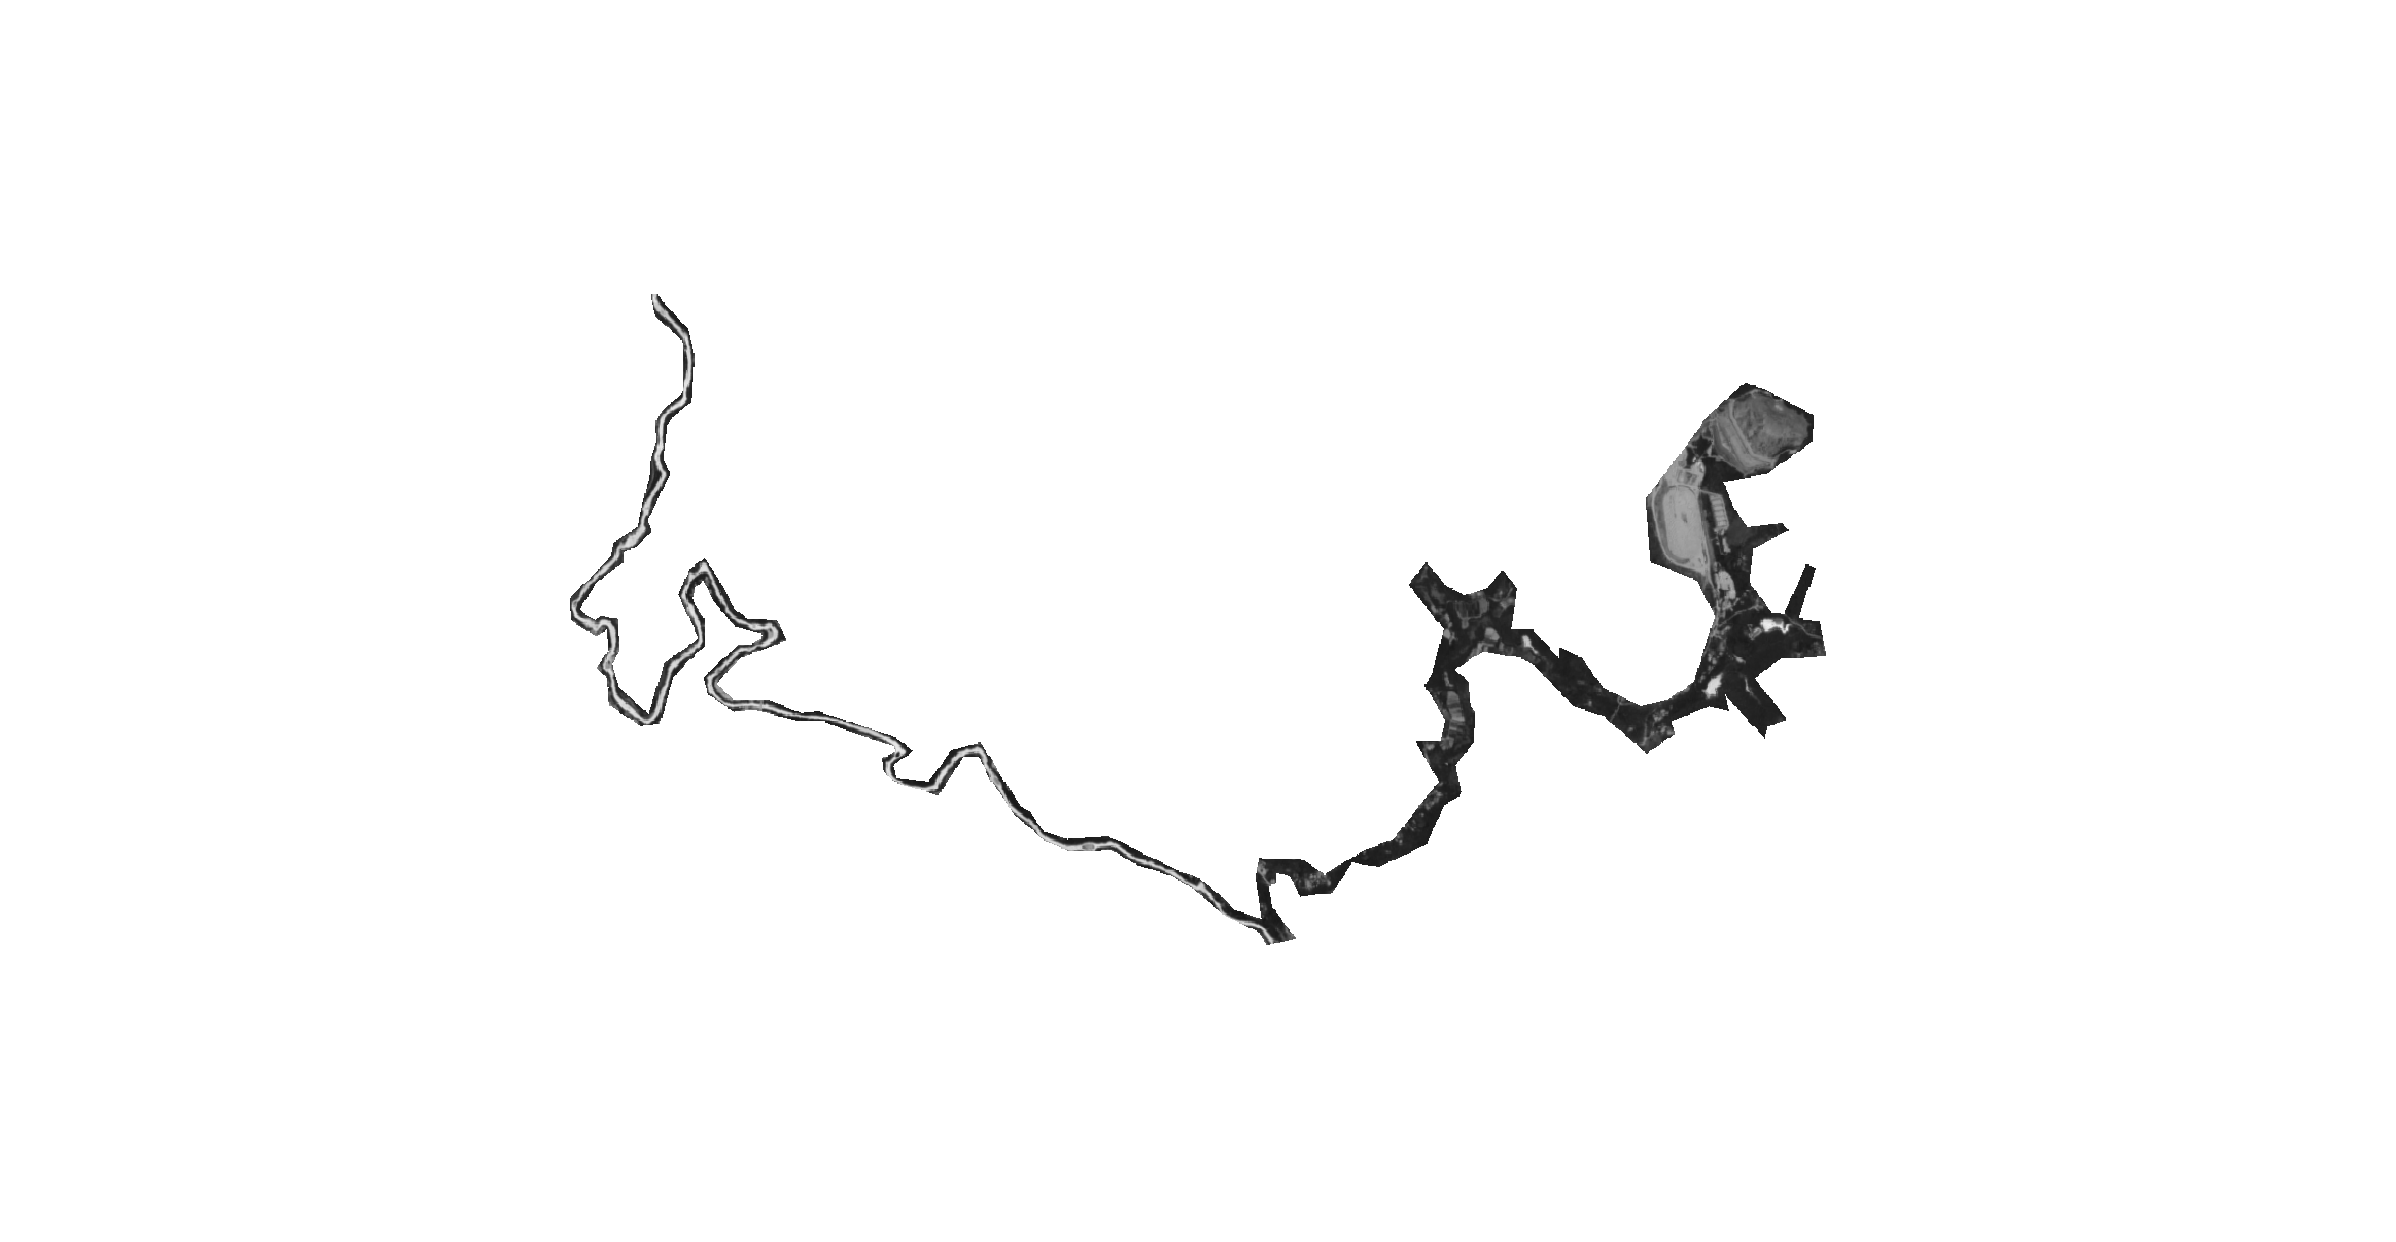
\includegraphics[width=\linewidth]{figures/ndvi_t1}\caption{NDVI $t_1$}\end{subfigure}
 \hfill
 \begin{subfigure}{0.49\textwidth}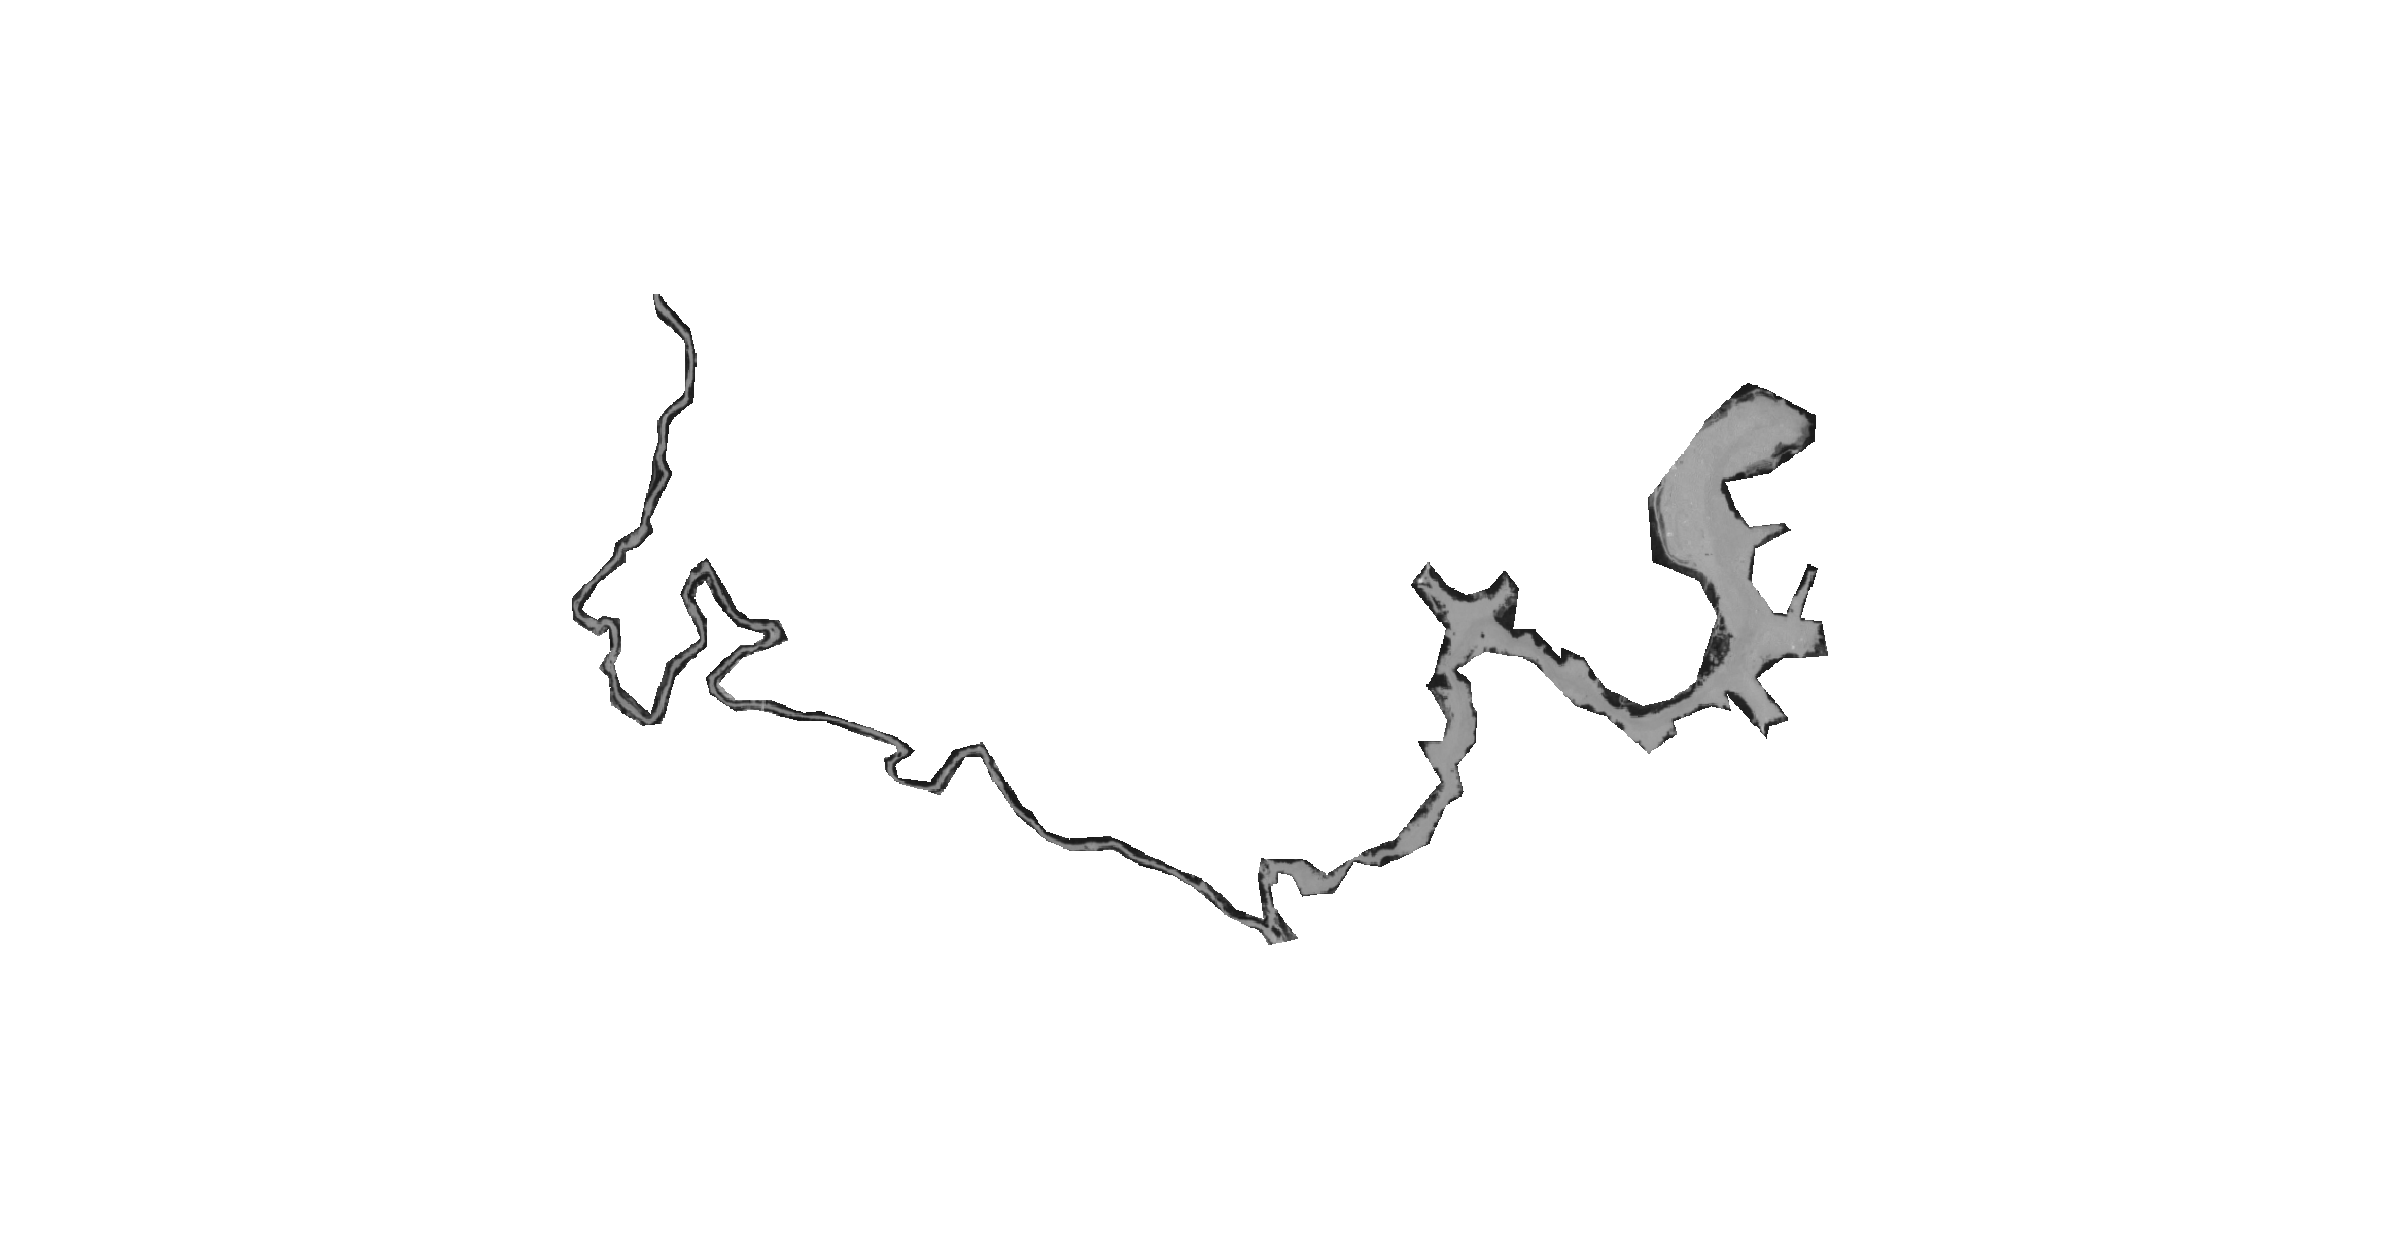
\includegraphics[width=\linewidth]{figures/ndvi_t2}\caption{NDVI $t_2$}\end{subfigure}
 \caption{NDVI antes y después del evento. Los tonos oscuros corresponden a NDVI alto (vegetación), los claros a NDVI bajo (suelo o material mineral) y los rojos a valores negativos (agua).}
 \label{fig:ndvi}
\end{figure}

\textbf{NDVI.} En $t_1$ (Figura~\ref{fig:ndvi}a) el corredor del Ribeirão Ferro-Carvão presenta tonos oscuros, es decir, NDVI alto, propio de vegetación riparia, fragmentos de bosque y pastos. Solo el sector de la mina muestra valores bajos, por tratarse de superficies de material expuesto. En $t_2$ (Figura~\ref{fig:ndvi}b) todo el corredor pasa a tonos claros, con NDVI cercano a cero. Este es el comportamiento típico de una superficie sin cobertura vegetal: el material depositado tiene una reflectancia en el rojo comparable a la del NIR. En el río Paraopeba los valores negativos se intensifican en $t_2$, lo que indica un cambio en las propiedades ópticas del agua.

\begin{figure}[H]
 \centering
 \begin{subfigure}{0.49\textwidth}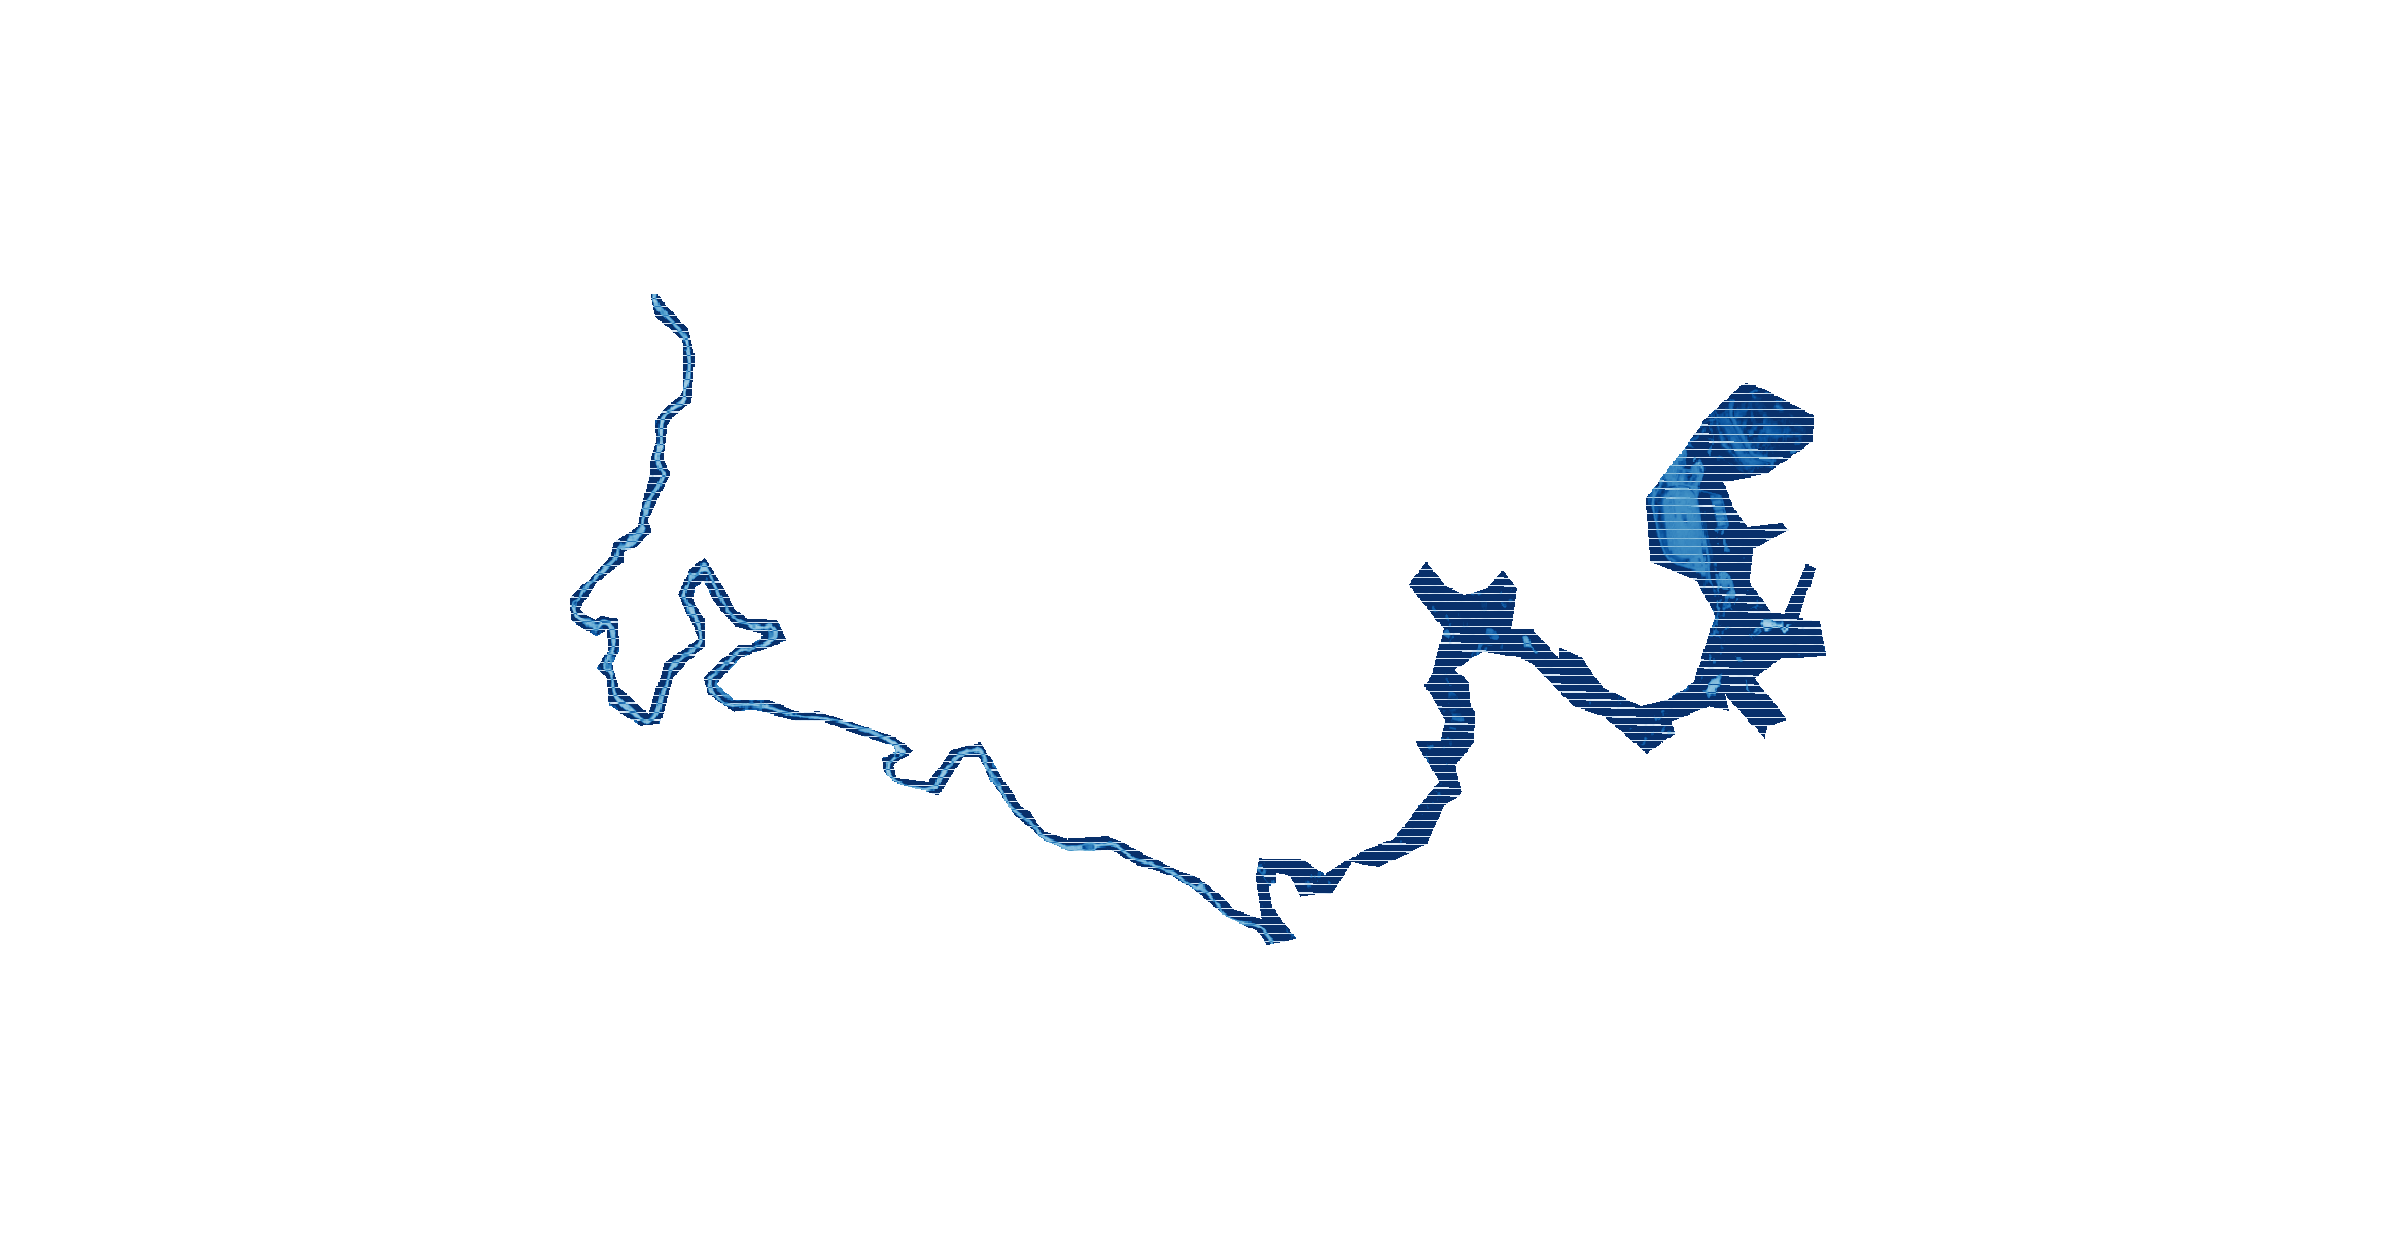
\includegraphics[width=\linewidth]{figures/ndwi_t1}\caption{NDWI $t_1$}\end{subfigure}
 \hfill
 \begin{subfigure}{0.49\textwidth}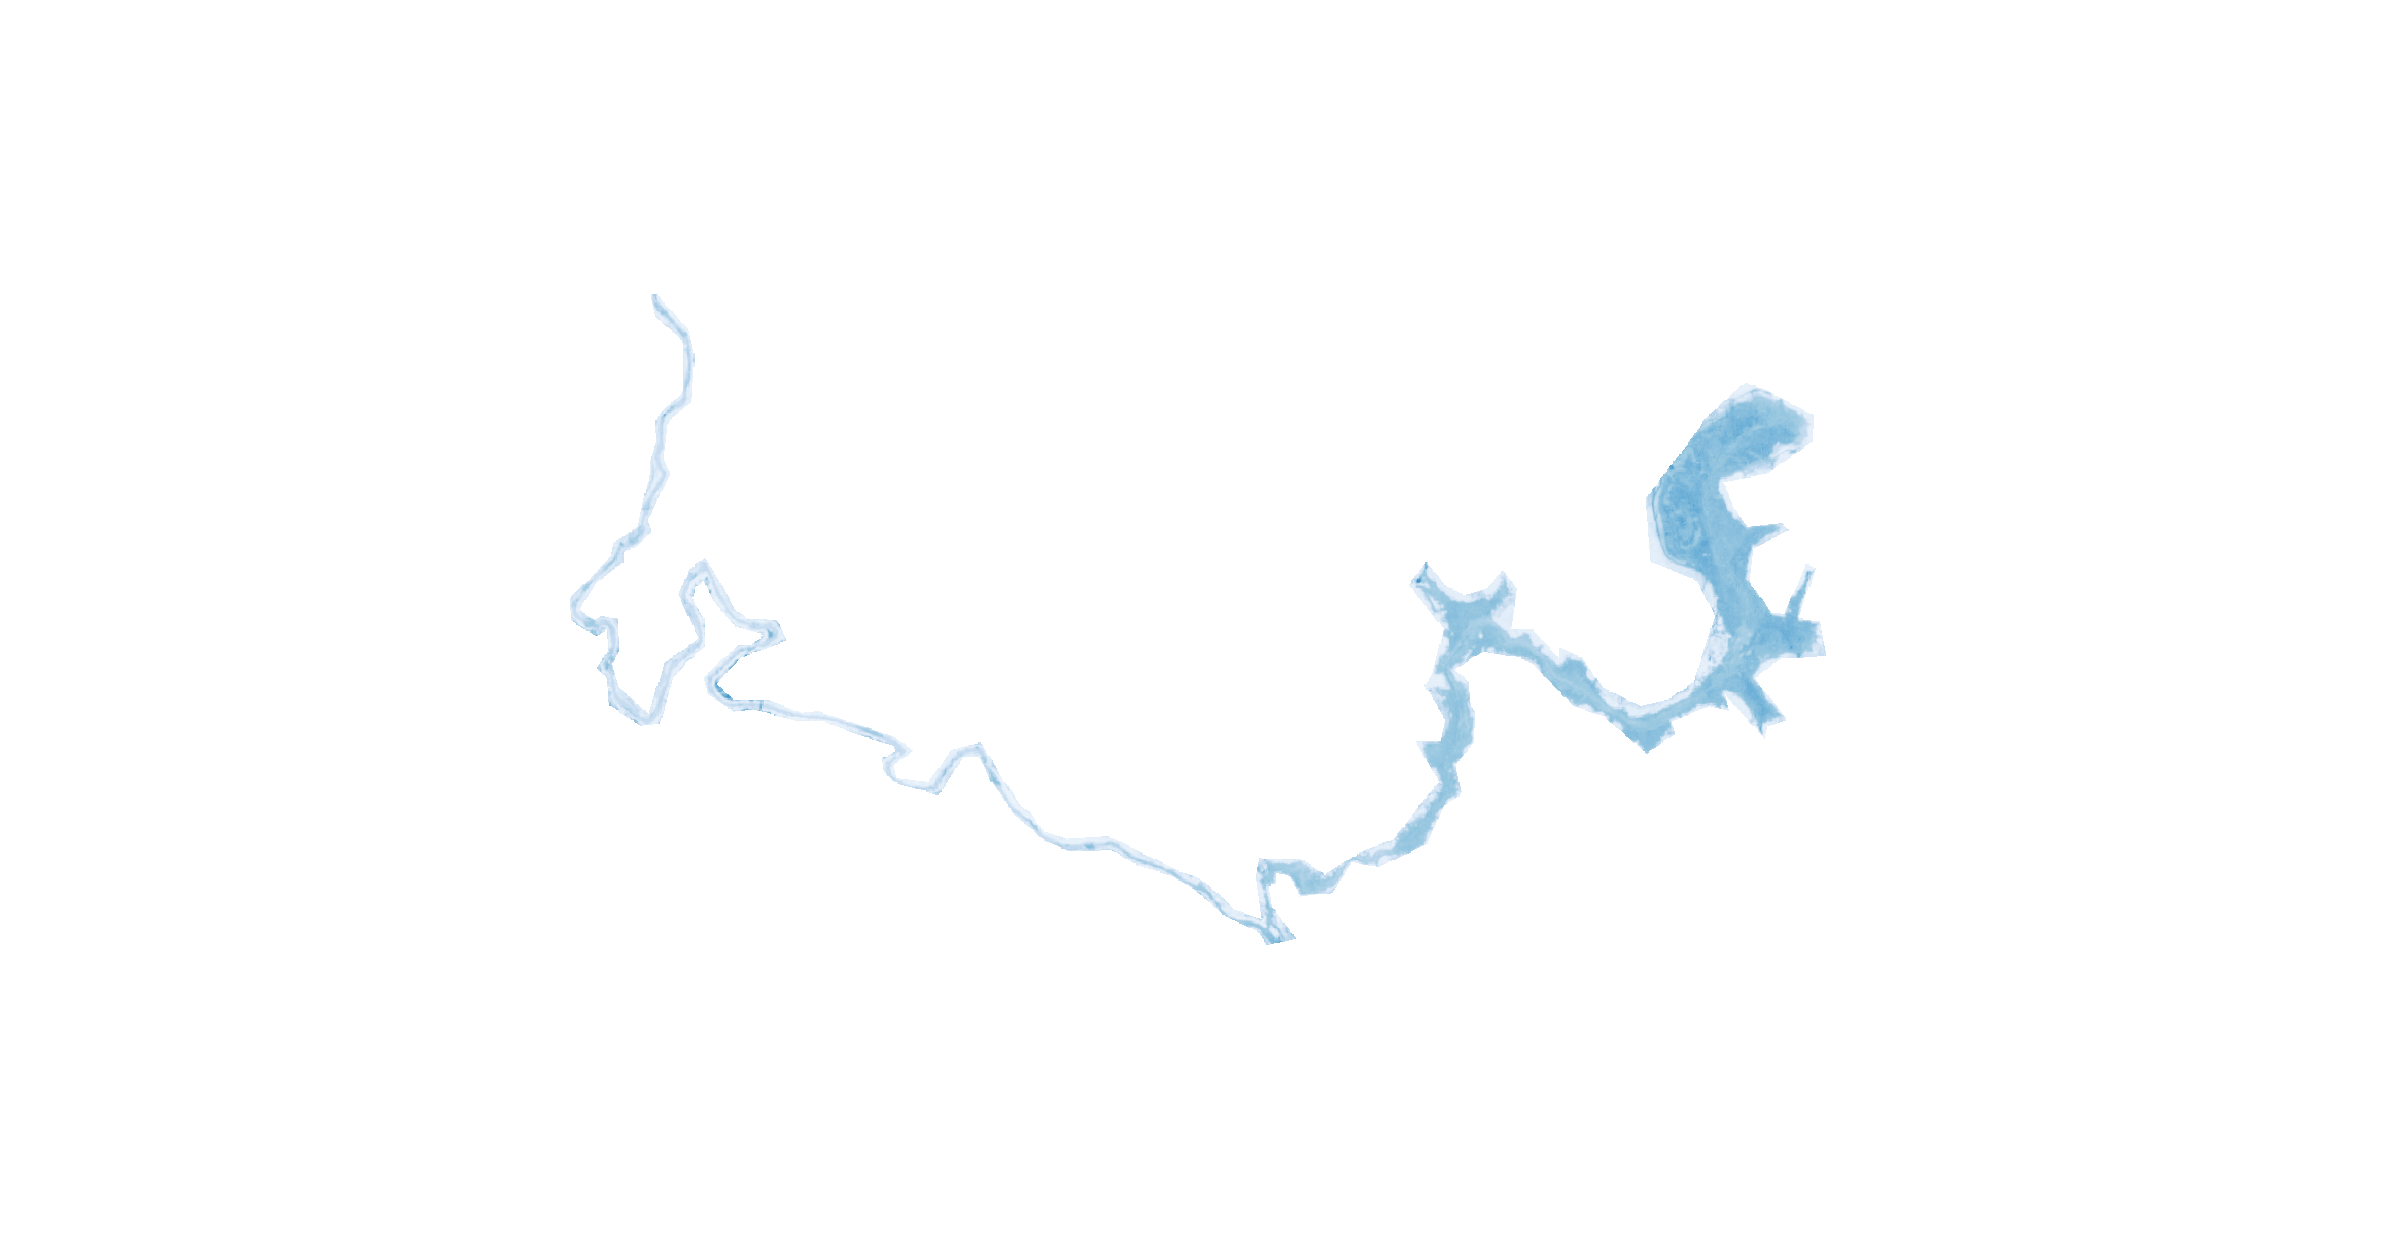
\includegraphics[width=\linewidth]{figures/ndwi_t2}\caption{NDWI $t_2$}\end{subfigure}
 \caption{NDWI antes y después del evento. Los azules más intensos indican valores más altos, asociados a agua superficial.}
 \label{fig:ndwi}
\end{figure}

\textbf{NDWI.} En ambas fechas (Figura~\ref{fig:ndwi}) los valores más altos se concentran en el cauce del Paraopeba, en pequeños cuerpos de agua próximos a la mina y en el sector de la mina misma. En $t_2$ el índice varía entre $-0{,}824$ y $0{,}024$. El patrón espacial general se mantiene entre fechas: el NDWI responde sobre todo al agua abierta y cambia poco sobre el material depositado en el valle.

\begin{figure}[H]
 \centering
 \begin{subfigure}{0.49\textwidth}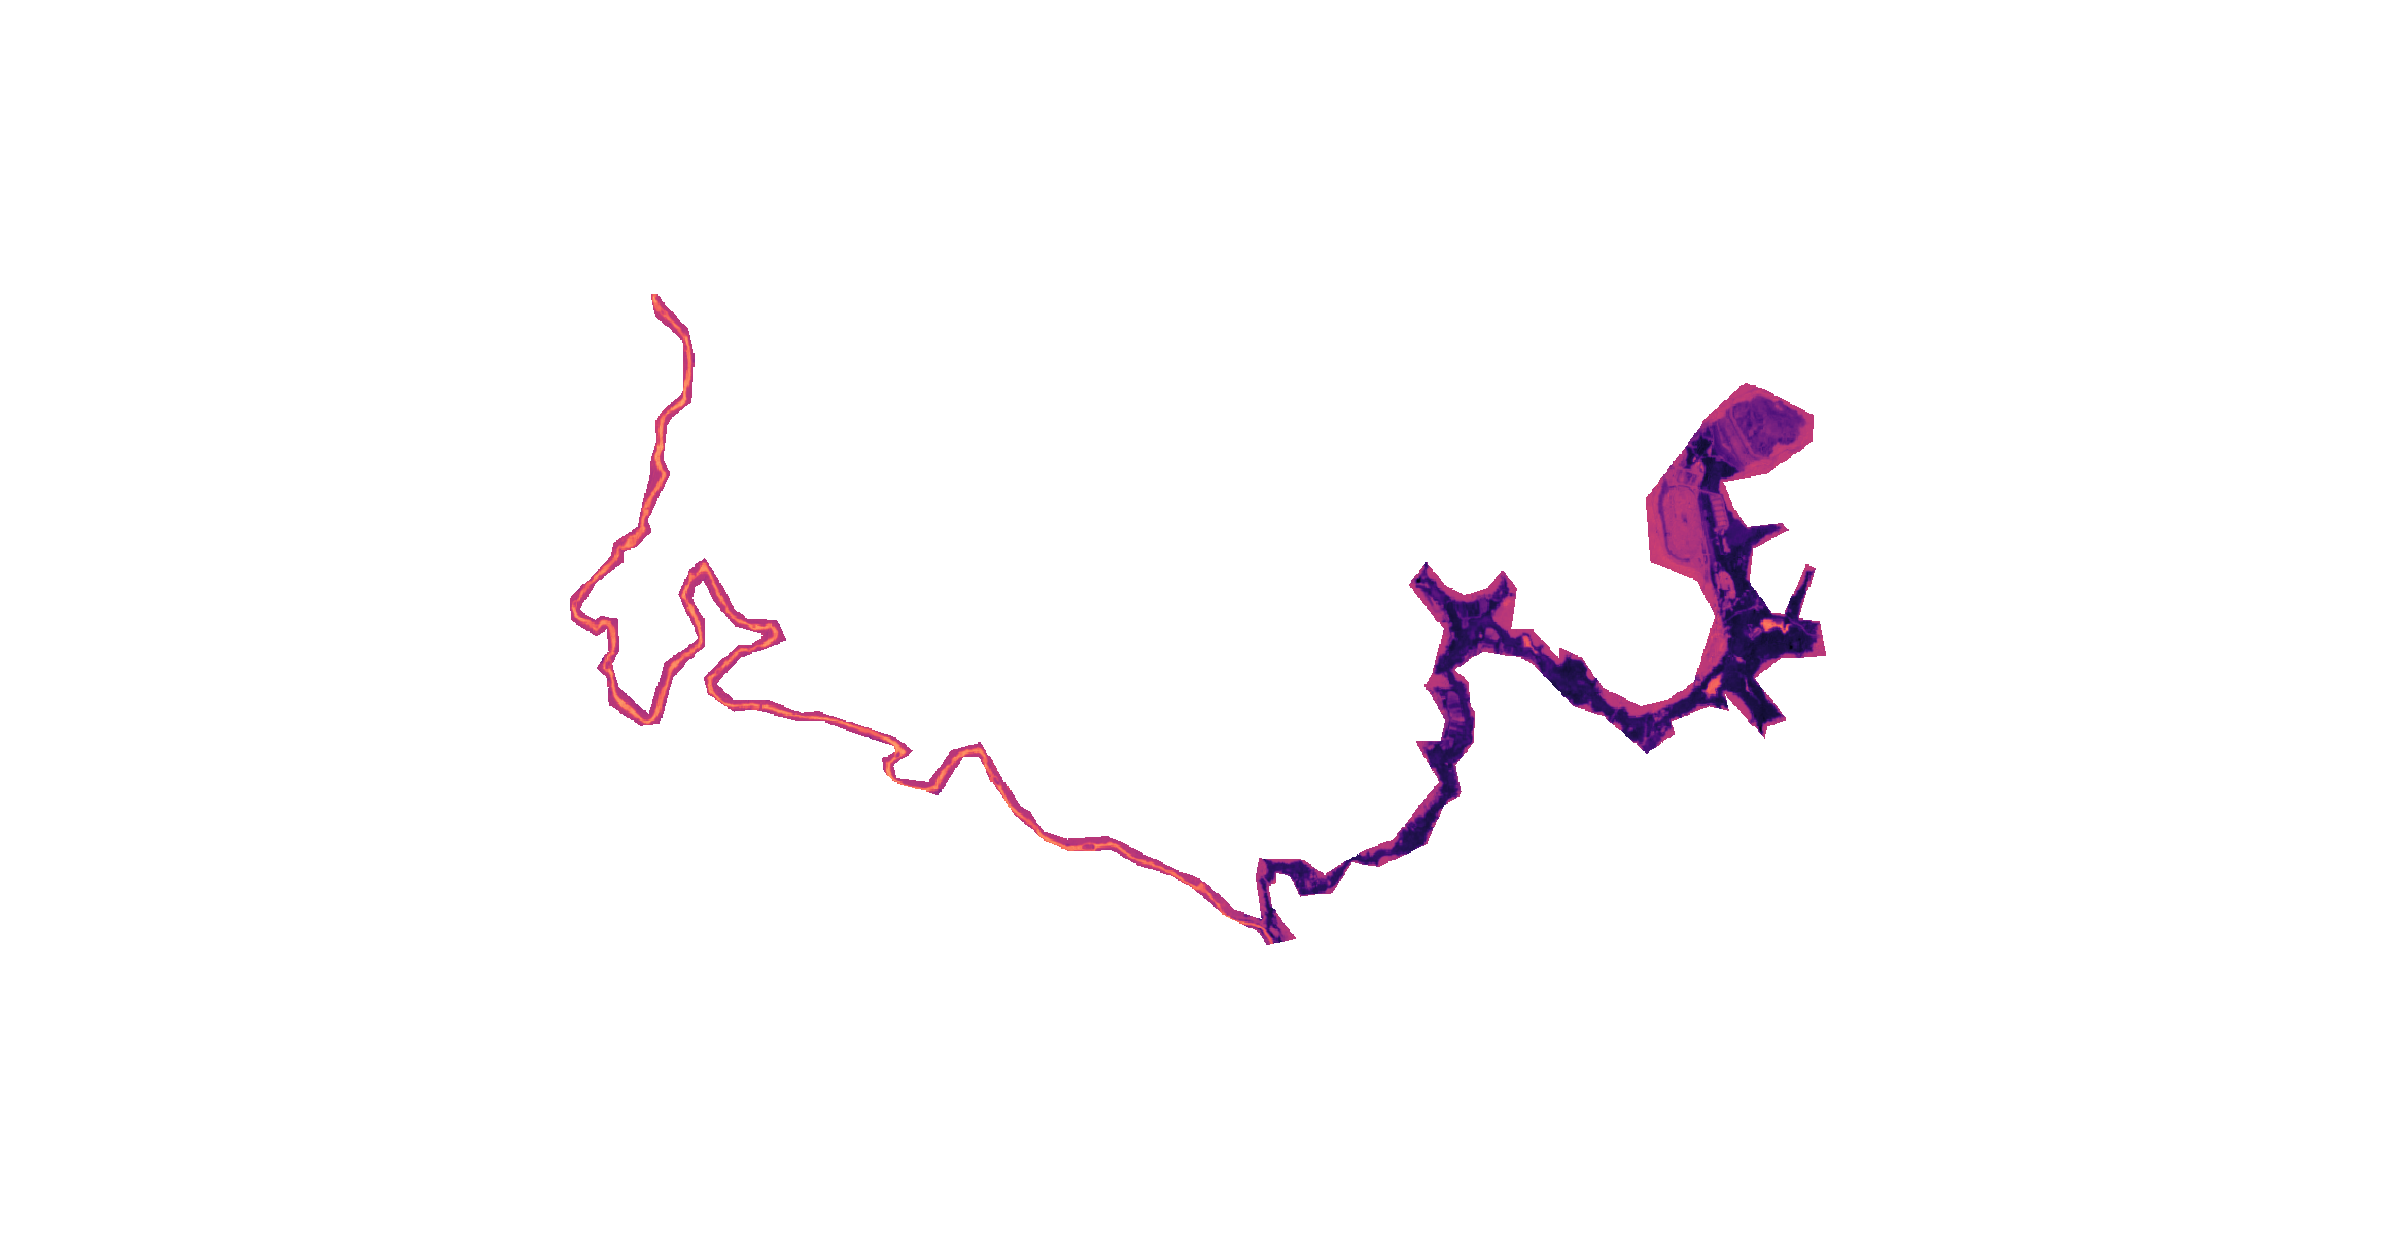
\includegraphics[width=\linewidth]{figures/dndvi}\caption{$\Delta$NDVI}\end{subfigure}
 \hfill
 \begin{subfigure}{0.49\textwidth}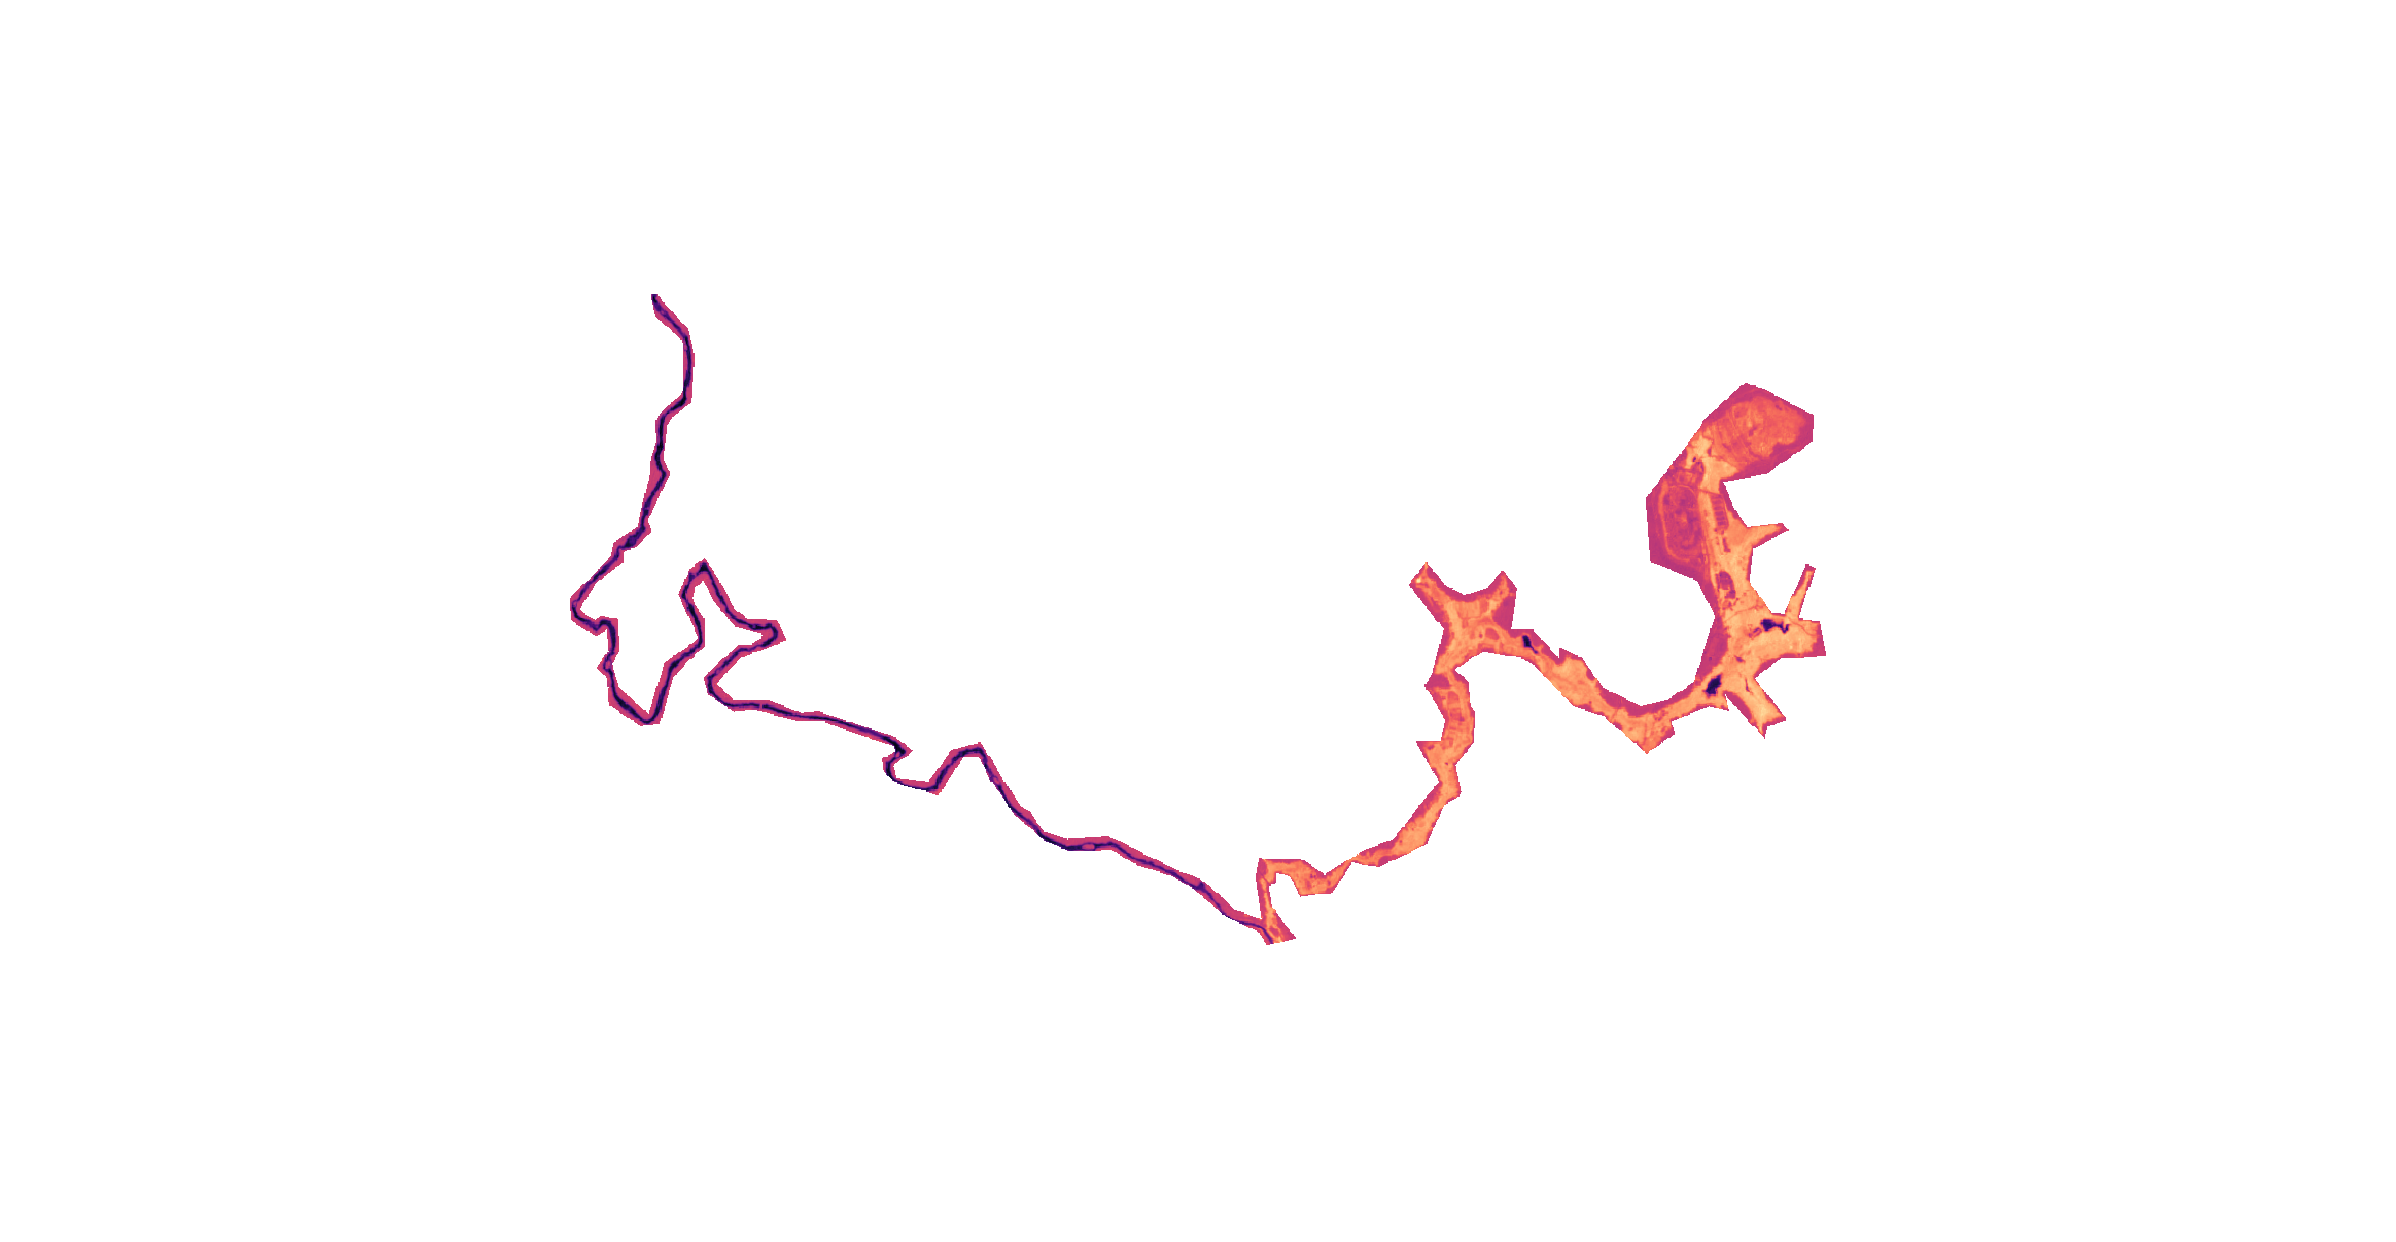
\includegraphics[width=\linewidth]{figures/dndwi}\caption{$\Delta$NDWI}\end{subfigure}
 \caption{Mapas de diferencia ($t_2 - t_1$). En $\Delta$NDVI los tonos oscuros indican la mayor disminución del índice.}
 \label{fig:delta}
\end{figure}

\textbf{$\Delta$NDVI.} El mapa de diferencia (Figura~\ref{fig:delta}a) está dominado por valores negativos, con un rango entre $-0{,}970$ y $0{,}771$. Las disminuciones más intensas se localizan en tres zonas:
\begin{enumerate}
    \item a lo largo del corredor del valle, desde el sector de la mina hasta la confluencia con el Paraopeba;
    \item en el cauce del Paraopeba, donde la mayor carga de sedimentos ricos en óxidos de hierro aumenta la reflectancia en el rojo;
    \item en el entorno inmediato de la mina.
\end{enumerate}
En los márgenes del ROI, fuera de la trayectoria del flujo, los valores son próximos a cero. Esto confirma que el cambio está espacialmente confinado al recorrido del material.

\textbf{$\Delta$NDWI.} La diferencia de NDWI (Figura~\ref{fig:delta}b) se concentra en el cauce y en el sector de la mina, con variaciones de menor magnitud que las de $\Delta$NDVI. El aumento de sólidos en suspensión eleva la reflectancia del agua tanto en el verde como en el NIR. Esto reduce el contraste en el que se basa el NDWI, de modo que la señal de agua persiste aunque su intensidad disminuye.

\subsection{Comparación entre NDVI y NDWI}
La Tabla~\ref{tab:comparacion} resume la respuesta de ambos índices según la zona.

\begin{table}[H]
 \centering
 \caption{Comparación de la respuesta de NDVI y NDWI por zona}
 \label{tab:comparacion}
 \begin{tabularx}{\textwidth}{lXX}
  \toprule
  \textbf{Zona} & \textbf{NDVI / $\Delta$NDVI} & \textbf{NDWI / $\Delta$NDWI} \\
  \midrule
  Corredor del valle & Disminución fuerte: transición de vegetación a material mineral. Es la señal de cambio más clara. & Cambio débil: el material depositado no se comporta como agua abierta. \\
  Río Paraopeba & Valores más negativos por el aumento de la reflectancia en el rojo asociado a sedimentos. & Se mantiene positivo (agua), con menor contraste por la turbidez. \\
  Sector de la mina & Valores bajos en ambas fechas; disminución en la vegetación circundante. & Variaciones asociadas a la redistribución de material húmedo. \\
  Fuera del flujo & $\Delta \approx 0$ & $\Delta \approx 0$ \\
  \bottomrule
 \end{tabularx}
\end{table}

La comparación muestra que el NDVI es el índice más discriminante para delimitar la huella del cambio. La transición de vegetación a material mineral produce el mayor contraste espectral entre fechas. El NDWI de McFeeters fue diseñado para agua abierta y responde de forma limitada a superficies de material saturado, pero aporta información complementaria sobre el comportamiento del cauce. En consecuencia, $\Delta$NDVI se adopta como variable principal para la umbralización de la Fase~4, y $\Delta$NDWI como variable de apoyo para el análisis del río.

\subsection{Estadísticas}
Los rangos observados de los índices son de $-0{,}824$ a $0{,}024$ para NDWI$_{t_2}$ y de $-0{,}970$ a $0{,}771$ para $\Delta$NDVI. La asimetría de este último rango, con una magnitud negativa alrededor de $1{,}3$ veces mayor que la positiva, indica que el cambio dominante en el ROI es la pérdida de vegetación. El cálculo del área total afectada (ha o km$^2$) se realizará en la Fase~4, una vez aplicada la umbralización y la vectorización.

\subsection{Discusión}
Los resultados muestran que una aproximación basada en índices espectrales, con imágenes de acceso libre y un preprocesamiento cuidadoso, permite identificar con claridad la trayectoria del material a lo largo del valle y su llegada al río Paraopeba. La corrección atmosférica (L2A), el co-registro verificado y la ausencia de nubes en el ROI respaldan que las diferencias observadas corresponden a cambios en la superficie y no a artefactos de adquisición.

Entre las limitaciones se cuenta una con que el NDWI de McFeeters es poco sensible a superficies húmedas no inundadas.

Para trabajos posteriores podría incorporarse el MNDWI con la banda SWIR (B11) o datos SAR de Sentinel-1.

\section{Conclusión}
\begin{itemize}
    \item Se construyó un par multitemporal Sentinel-2 L2A (17-01-2019 y 01-02-2019) radiométricamente comparable: corregido atmosféricamente, co-registrado píxel a píxel y sin nubes dentro del ROI según la máscara SCL.
    \item El NDVI y su diferencia delimitan con claridad la zona de cambio. La disminución del índice se concentra en el corredor del Ribeirão Ferro-Carvão y en el cauce del Paraopeba, mientras que las áreas fuera de la trayectoria permanecen estables.
    \item El NDWI identifica consistentemente el agua superficial, pero es menos sensible al material depositado. Su utilidad principal es complementar el análisis del río.
    \item La siguiente etapa aplicará umbralización, validación con imágenes de alta resolución, vectorización y cálculo del área afectada.
\end{itemize}

\printbibliography

\end{document}
